\PassOptionsToPackage{unicode=true}{hyperref} % options for packages loaded elsewhere
\PassOptionsToPackage{hyphens}{url}
%
\documentclass[]{book}
\usepackage{lmodern}
\usepackage{amssymb,amsmath}
\usepackage{ifxetex,ifluatex}
\usepackage{fixltx2e} % provides \textsubscript
\ifnum 0\ifxetex 1\fi\ifluatex 1\fi=0 % if pdftex
  \usepackage[T1]{fontenc}
  \usepackage[utf8]{inputenc}
  \usepackage{textcomp} % provides euro and other symbols
\else % if luatex or xelatex
  \usepackage{unicode-math}
  \defaultfontfeatures{Ligatures=TeX,Scale=MatchLowercase}
\fi
% use upquote if available, for straight quotes in verbatim environments
\IfFileExists{upquote.sty}{\usepackage{upquote}}{}
% use microtype if available
\IfFileExists{microtype.sty}{%
\usepackage[]{microtype}
\UseMicrotypeSet[protrusion]{basicmath} % disable protrusion for tt fonts
}{}
\IfFileExists{parskip.sty}{%
\usepackage{parskip}
}{% else
\setlength{\parindent}{0pt}
\setlength{\parskip}{6pt plus 2pt minus 1pt}
}
\usepackage{hyperref}
\hypersetup{
            pdftitle={RJafroc Documentation},
            pdfauthor={Dev P. Chakraborty, PhD},
            pdfborder={0 0 0},
            breaklinks=true}
\urlstyle{same}  % don't use monospace font for urls
\usepackage{color}
\usepackage{fancyvrb}
\newcommand{\VerbBar}{|}
\newcommand{\VERB}{\Verb[commandchars=\\\{\}]}
\DefineVerbatimEnvironment{Highlighting}{Verbatim}{commandchars=\\\{\}}
% Add ',fontsize=\small' for more characters per line
\usepackage{framed}
\definecolor{shadecolor}{RGB}{248,248,248}
\newenvironment{Shaded}{\begin{snugshade}}{\end{snugshade}}
\newcommand{\AlertTok}[1]{\textcolor[rgb]{0.94,0.16,0.16}{#1}}
\newcommand{\AnnotationTok}[1]{\textcolor[rgb]{0.56,0.35,0.01}{\textbf{\textit{#1}}}}
\newcommand{\AttributeTok}[1]{\textcolor[rgb]{0.77,0.63,0.00}{#1}}
\newcommand{\BaseNTok}[1]{\textcolor[rgb]{0.00,0.00,0.81}{#1}}
\newcommand{\BuiltInTok}[1]{#1}
\newcommand{\CharTok}[1]{\textcolor[rgb]{0.31,0.60,0.02}{#1}}
\newcommand{\CommentTok}[1]{\textcolor[rgb]{0.56,0.35,0.01}{\textit{#1}}}
\newcommand{\CommentVarTok}[1]{\textcolor[rgb]{0.56,0.35,0.01}{\textbf{\textit{#1}}}}
\newcommand{\ConstantTok}[1]{\textcolor[rgb]{0.00,0.00,0.00}{#1}}
\newcommand{\ControlFlowTok}[1]{\textcolor[rgb]{0.13,0.29,0.53}{\textbf{#1}}}
\newcommand{\DataTypeTok}[1]{\textcolor[rgb]{0.13,0.29,0.53}{#1}}
\newcommand{\DecValTok}[1]{\textcolor[rgb]{0.00,0.00,0.81}{#1}}
\newcommand{\DocumentationTok}[1]{\textcolor[rgb]{0.56,0.35,0.01}{\textbf{\textit{#1}}}}
\newcommand{\ErrorTok}[1]{\textcolor[rgb]{0.64,0.00,0.00}{\textbf{#1}}}
\newcommand{\ExtensionTok}[1]{#1}
\newcommand{\FloatTok}[1]{\textcolor[rgb]{0.00,0.00,0.81}{#1}}
\newcommand{\FunctionTok}[1]{\textcolor[rgb]{0.00,0.00,0.00}{#1}}
\newcommand{\ImportTok}[1]{#1}
\newcommand{\InformationTok}[1]{\textcolor[rgb]{0.56,0.35,0.01}{\textbf{\textit{#1}}}}
\newcommand{\KeywordTok}[1]{\textcolor[rgb]{0.13,0.29,0.53}{\textbf{#1}}}
\newcommand{\NormalTok}[1]{#1}
\newcommand{\OperatorTok}[1]{\textcolor[rgb]{0.81,0.36,0.00}{\textbf{#1}}}
\newcommand{\OtherTok}[1]{\textcolor[rgb]{0.56,0.35,0.01}{#1}}
\newcommand{\PreprocessorTok}[1]{\textcolor[rgb]{0.56,0.35,0.01}{\textit{#1}}}
\newcommand{\RegionMarkerTok}[1]{#1}
\newcommand{\SpecialCharTok}[1]{\textcolor[rgb]{0.00,0.00,0.00}{#1}}
\newcommand{\SpecialStringTok}[1]{\textcolor[rgb]{0.31,0.60,0.02}{#1}}
\newcommand{\StringTok}[1]{\textcolor[rgb]{0.31,0.60,0.02}{#1}}
\newcommand{\VariableTok}[1]{\textcolor[rgb]{0.00,0.00,0.00}{#1}}
\newcommand{\VerbatimStringTok}[1]{\textcolor[rgb]{0.31,0.60,0.02}{#1}}
\newcommand{\WarningTok}[1]{\textcolor[rgb]{0.56,0.35,0.01}{\textbf{\textit{#1}}}}
\usepackage{longtable,booktabs}
% Fix footnotes in tables (requires footnote package)
\IfFileExists{footnote.sty}{\usepackage{footnote}\makesavenoteenv{longtable}}{}
\usepackage{graphicx,grffile}
\makeatletter
\def\maxwidth{\ifdim\Gin@nat@width>\linewidth\linewidth\else\Gin@nat@width\fi}
\def\maxheight{\ifdim\Gin@nat@height>\textheight\textheight\else\Gin@nat@height\fi}
\makeatother
% Scale images if necessary, so that they will not overflow the page
% margins by default, and it is still possible to overwrite the defaults
% using explicit options in \includegraphics[width, height, ...]{}
\setkeys{Gin}{width=\maxwidth,height=\maxheight,keepaspectratio}
\setlength{\emergencystretch}{3em}  % prevent overfull lines
\providecommand{\tightlist}{%
  \setlength{\itemsep}{0pt}\setlength{\parskip}{0pt}}
\setcounter{secnumdepth}{5}
% Redefines (sub)paragraphs to behave more like sections
\ifx\paragraph\undefined\else
\let\oldparagraph\paragraph
\renewcommand{\paragraph}[1]{\oldparagraph{#1}\mbox{}}
\fi
\ifx\subparagraph\undefined\else
\let\oldsubparagraph\subparagraph
\renewcommand{\subparagraph}[1]{\oldsubparagraph{#1}\mbox{}}
\fi

% set default figure placement to htbp
\makeatletter
\def\fps@figure{htbp}
\makeatother

\usepackage{booktabs}
\usepackage{amsthm}
\makeatletter
\def\thm@space@setup{%
  \thm@preskip=8pt plus 2pt minus 4pt
  \thm@postskip=\thm@preskip
}
\makeatother
\usepackage[]{natbib}
\bibliographystyle{apalike}

\title{RJafroc Documentation}
\author{Dev P. Chakraborty, PhD}
\date{2020-03-10}

\begin{document}
\maketitle

{
\setcounter{tocdepth}{1}
\tableofcontents
}
\hypertarget{preface}{%
\chapter*{Preface}\label{preface}}
\addcontentsline{toc}{chapter}{Preface}

\begin{itemize}
\tightlist
\item
  This book, an extended documentation of the \textbf{RJafroc} package, is undergoing extensive edits.
\item
  It should not be used by the casual user until I give the go ahead.
\item
  It bypasses the file size limits of \textbf{CRAN}, currently 5 MB, which severely limits the extent of the documentation that can be included with the CRAN version of the package.
\item
  I welcome corrections and comments by the not-so-casual-user.
\item
  Please use the GitHub website to raise issues and comments:

  \begin{itemize}
  \tightlist
  \item
    \url{https://github.com/dpc10ster/RJafrocBook}
  \end{itemize}
\end{itemize}

\hypertarget{intro}{%
\chapter{Introduction}\label{intro}}

\begin{itemize}
\tightlist
\item
  This is the book desribing the \textbf{RJafroc} package.
\item
  The name of the book is RJafrocBook
\item
  Modality and treatment are used interchangeably.
\item
  Reader is a generic radiologist, or a computer aided detection algorithm, or any algorithmic ``reader''
\item
  TBA
\end{itemize}

\hypertarget{rocdataformat}{%
\chapter{ROC data format}\label{rocdataformat}}

\hypertarget{introduction}{%
\section{Introduction}\label{introduction}}

\begin{itemize}
\tightlist
\item
  The purpose of this vignette is to explain the data format of the input Excel file and to introduce the capabilities of the function \texttt{DfReadDataFile()}. Background on observer performance methods are in my book \citep{RN2680}.
\item
  I will start with Receiver Operating Characteristic (ROC) data \citep{RN1766}, as this is by far the simplest paradigm.
\item
  In the ROC paradigm the observer assigns a rating to each image. A rating is an ordered numeric label, and, in our convention, higher values represent greater certainty or \textbf{confidence level} for presence of disease. With human observers, a 5 (or 6) point rating scale is typically used, with 1 representing highest confidence for \emph{absence} of disease and 5 (or 6) representing highest confidence for \emph{presence} of disease. Intermediate values represent intermediate confidence levels for presence or absence of disease.
\item
  Note that location information associated with the disease, if applicable, is not collected.
\item
  There is no restriction to 5 or 6 ratings. With algorithmic observers, e.g., computer aided detection (CAD) algorithms, the rating could be a floating point number and have infinite precision. All that is required is that higher values correspond to greater confidence in presence of disease.
\end{itemize}

\hypertarget{note-to-existing-users}{%
\section{Note to existing users}\label{note-to-existing-users}}

\begin{itemize}
\tightlist
\item
  The Excel file format has recently undergone changes resulting in 4 extra \texttt{list} members in the final created \texttt{dataset} object (i.e., 12 members instead of 8).
\item
  Code should run on the old format Excel files as the 4 extra list members are simply ignored.
\item
  Reasons for the change will become clearer in these vignettes
\item
  Basically they are needed for generalization to other data collection paradigms instead of crossed, for example to the split-plot data acquisition paradigm, and for better data entry error control.
\end{itemize}

\hypertarget{the-excel-data-format}{%
\section{The Excel data format}\label{the-excel-data-format}}

\begin{itemize}
\tightlist
\item
  The Excel file has three worksheets.
\item
  These are named

  \begin{itemize}
  \tightlist
  \item
    \texttt{Truth},
  \item
    \texttt{NL} (or \texttt{FP}),
  \item
    \texttt{LL} (or \texttt{TP}).
  \end{itemize}
\end{itemize}

\hypertarget{illustrative-toy-file}{%
\section{Illustrative toy file}\label{illustrative-toy-file}}

\begin{itemize}
\tightlist
\item
  \emph{Toy files} are artificial small datasets intended to illustrate essential features of the data format.\\
\item
  The examples shown in this vignette corresponds to Excel file \texttt{inst/extdata/toyFiles/ROC/rocCr.xlsx} in the project directory.
\item
  To view these files one needs to \texttt{clone} the source files from \texttt{GitHub}.
\end{itemize}

\hypertarget{the-truth-worksheet}{%
\section{\texorpdfstring{The \texttt{Truth} worksheet}{The Truth worksheet}}\label{the-truth-worksheet}}

\begin{itemize}
\tightlist
\item
  The \texttt{Truth} worksheet contains 6 columns: \texttt{CaseID}, \texttt{LesionID}, \texttt{Weight}, \texttt{ReaderID}, \texttt{ModalityID} and \texttt{Paradigm}.
\item
  For ROC data the first five columns contain as many rows as there are cases (images) in the dataset.
\item
  \texttt{CaseID}: unique integers, one per case, representing the cases in the dataset.
\item
  \texttt{LesionID}: integers 0 or 1, with each 0 representing a non-diseased case and each 1 representing a diseased case.
\item
  In the current toy dataset, the non-diseased cases are labeled \texttt{1}, \texttt{2} and \texttt{3}, while the diseased cases are labeled \texttt{70}, \texttt{71}, \texttt{72}, \texttt{73} and \texttt{74}. The values do not have to be consecutive integers; they need not be ordered; the only requirement is that they be \textbf{unique}.
\item
  \texttt{Weight}: Not used for ROC data, a floating point value, typically filled in with 0 or 1.
\item
  \texttt{ReaderID}: a \textbf{comma-separated} listing of reader labels, each represented by a \textbf{unique string}, that have interpreted the case. In the example shown below each cell has the value \texttt{0,\ 1,\ 2,\ 3,\ 4} meaning that each of the readers, represented by the strings ``0'', ``1'', ``2'', ``3'' and ``4'', have interpreted all cases (hence the ``crossed'' design). \textbf{With reader names that could be confused with integers, each cell in this column has to be text formatted as otherwise Excel will not accept it.} {[}Try entering \texttt{0,\ 1,\ 2,\ 3,\ 4} in a numeric formatted Excel cell.{]}
\item
  The reader names could just as well have been \texttt{Rdr0,\ Rdr1,\ Rdr2,\ Rdr3,\ Rdr4}. The only requirement is that they be unique strings.
\item
  Look in in the \texttt{inst/extdata/toyFiles/ROC} directory for files \texttt{rocCrStrRdrsTrts.xlsx} and \texttt{rocCrStrRdrsNonUnique.xlsx} for examples of data files using longer strings for readers. The second file generates an error because the reader names are not unique.
\item
  \texttt{ModalityID}: a comma-separated listing of modalities (one or more modalities), each represented by a \textbf{unique string}, that are applied to each case. In the example each cell has the value \texttt{"0",\ "1"}. \textbf{With treatment names that could be confused with integers, each cell has to be text formatted as otherwise Excel will not accept it.}
\item
  The treatment names could just as well have been \texttt{Trt0,\ Trt1}. Again, the only requirement is that they be unique strings.
\item
  \texttt{Paradigm}: this column contains two cells, \texttt{ROC} and \texttt{crossed}. It informs the software that this is an ROC dataset, and the design is crossed, meaning each reader has interpreted each case in each modality (in statistical terminology: modality and reader factors are ``crossed'').
\item
  There are 5 diseased cases in the dataset (the number of 1's in the \texttt{LesionID} column of the \texttt{Truth} worksheet).
\item
  There are 3 non-diseased cases in the dataset (the number of 0's in the \texttt{LesionID} column).
\item
  There are 5 readers in the dataset (each cell in the \texttt{ReaderID} column contains the string \texttt{0,\ 1,\ 2,\ 3,\ 4}).
\item
  There are 2 modalities in the dataset (each cell in the \texttt{ModalityID} column contains the string \texttt{0,\ 1}).
\end{itemize}

\begin{figure}

{\centering 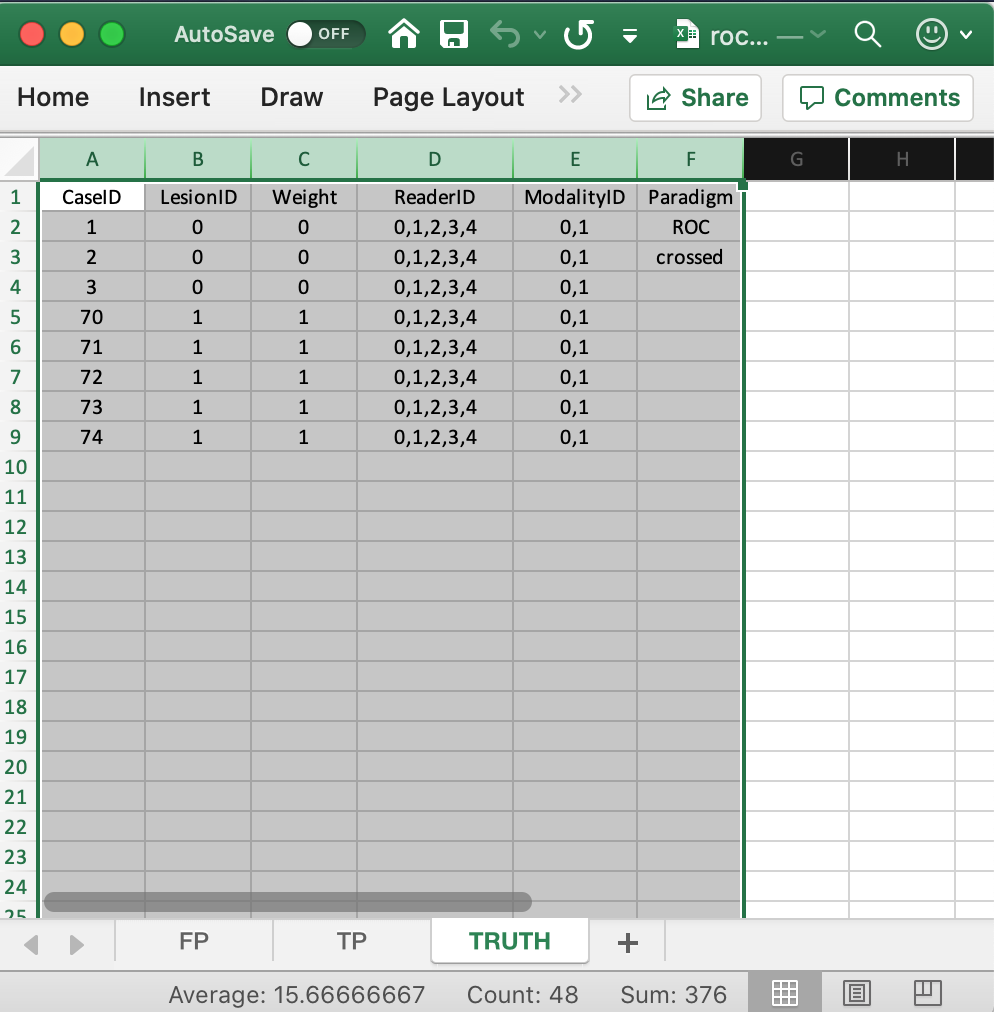
\includegraphics[width=0.5\linewidth,height=0.2\textheight]{images/rocCrTruth} 

}

\caption{Truth worksheet for file rocCr.xlsx}\label{fig:showRocCrTruthSheet}
\end{figure}

\hypertarget{the-structure-of-an-roc-dataset}{%
\section{The structure of an ROC dataset}\label{the-structure-of-an-roc-dataset}}

In the following code chunk the first statement retrieves the name of the data file, located in a hidden directory that one need not be concerned with. The second statement reads the file using the function \texttt{DfReadDataFile()} and saves it to object \texttt{x}. The third statement shows the structure of the dataset object \texttt{x}.

\begin{Shaded}
\begin{Highlighting}[]
\NormalTok{rocCr <-}\StringTok{ }\KeywordTok{system.file}\NormalTok{(}\StringTok{"extdata"}\NormalTok{, }\StringTok{"toyFiles/ROC/rocCr.xlsx"}\NormalTok{,}
                        \DataTypeTok{package =} \StringTok{"RJafroc"}\NormalTok{, }\DataTypeTok{mustWork =} \OtherTok{TRUE}\NormalTok{)}
\NormalTok{x <-}\StringTok{ }\KeywordTok{DfReadDataFile}\NormalTok{(rocCr, }\DataTypeTok{newExcelFileFormat =} \OtherTok{TRUE}\NormalTok{)}
\KeywordTok{str}\NormalTok{(x)}
\CommentTok{#> List of 12}
\CommentTok{#>  $ NL           : num [1:2, 1:5, 1:8, 1] 1 3 2 3 2 2 1 2 3 2 ...}
\CommentTok{#>  $ LL           : num [1:2, 1:5, 1:5, 1] 5 5 5 5 5 5 5 5 5 5 ...}
\CommentTok{#>  $ lesionVector : int [1:5] 1 1 1 1 1}
\CommentTok{#>  $ lesionID     : num [1:5, 1] 1 1 1 1 1}
\CommentTok{#>  $ lesionWeight : num [1:5, 1] 1 1 1 1 1}
\CommentTok{#>  $ dataType     : chr "ROC"}
\CommentTok{#>  $ modalityID   : Named chr [1:2] "0" "1"}
\CommentTok{#>   ..- attr(*, "names")= chr [1:2] "0" "1"}
\CommentTok{#>  $ readerID     : Named chr [1:5] "0" "1" "2" "3" ...}
\CommentTok{#>   ..- attr(*, "names")= chr [1:5] "0" "1" "2" "3" ...}
\CommentTok{#>  $ design       : chr "CROSSED"}
\CommentTok{#>  $ normalCases  : int [1:3] 1 2 3}
\CommentTok{#>  $ abnormalCases: int [1:5] 70 71 72 73 74}
\CommentTok{#>  $ truthTableStr: num [1:2, 1:5, 1:8, 1:2] 1 1 1 1 1 1 1 1 1 1 ...}
\end{Highlighting}
\end{Shaded}

\begin{itemize}
\tightlist
\item
  In the above code chunk flag \texttt{newExcelFileFormat} is set to \texttt{TRUE} as otherwise columns D - F in the \texttt{Truth} worksheet are ignored and the dataset is assumed to be crossed, with \texttt{dataType} automatically determined from the contents of the FP and TP worksheets.
\item
  Flag \texttt{newExcelFileFormat\ =\ FALSE} is for compatibility with older JAFROC format Excel files, which did not have these columns in the \texttt{Truth} worksheet. Its usage is deprecated.
\item
  The dataset object \texttt{x} is a \texttt{list} variable with 12 members.
\item
  The \texttt{x\$NL} member, with dimension {[}2, 5, 8, 1{]}, contains the ratings of normal cases. The extra values in the third dimension, filled with \texttt{NAs}, are needed for compatibility with FROC datasets, as unlike ROC, false positives are possible on diseased cases.
\item
  The \texttt{x\$LL}, with dimension {[}2, 5, 5, 1{]}, contains the ratings of abnormal cases.
\item
  The \texttt{x\$lesionVector} member is a vector with 5 ones representing the 5 diseased cases in the dataset.
\item
  The \texttt{x\$lesionID} member is an array with 5 ones.
\item
  The \texttt{x\$lesionWeight} member is an array with 5 ones.
\item
  The \texttt{lesionVector}, \texttt{lesionID} and \texttt{lesionWeight} members are not used for ROC datasets. They are there for compatibility with FROC datasets.
\item
  The \texttt{dataType} member indicates that this is an \texttt{ROC} dataset.
\item
  The \texttt{x\$modalityID} member is a vector with two elements \texttt{"0"} and \texttt{"1"}, naming the two modalities.
\item
  The \texttt{x\$readerID} member is a vector with five elements \texttt{"0"}, \texttt{"1"}, \texttt{"2"}, \texttt{"3"} and \texttt{"4"}, naming the five readers.
\item
  The \texttt{x\$design} member is CROSSED; specifies the dataset design, which is ``CROSSED''.
\item
  The \texttt{x\$normalCases} member lists the integer names of the normal cases, 1, 2, 3.
\item
  The \texttt{x\$abnormalCases} member lists the integer names of the abnormal cases, 70, 71, 72, 73, 74.
\item
  The \texttt{x\$truthTableStr} member quantifies the structure of the dataset, as explained in \textbf{Chapter 00 Vignette \#3-\#5}.
\end{itemize}

\hypertarget{the-false-positive-fp-ratings}{%
\section{The false positive (FP) ratings}\label{the-false-positive-fp-ratings}}

These are found in the \texttt{FP} or \texttt{NL} worksheet, see below.

\begin{figure}

{\centering 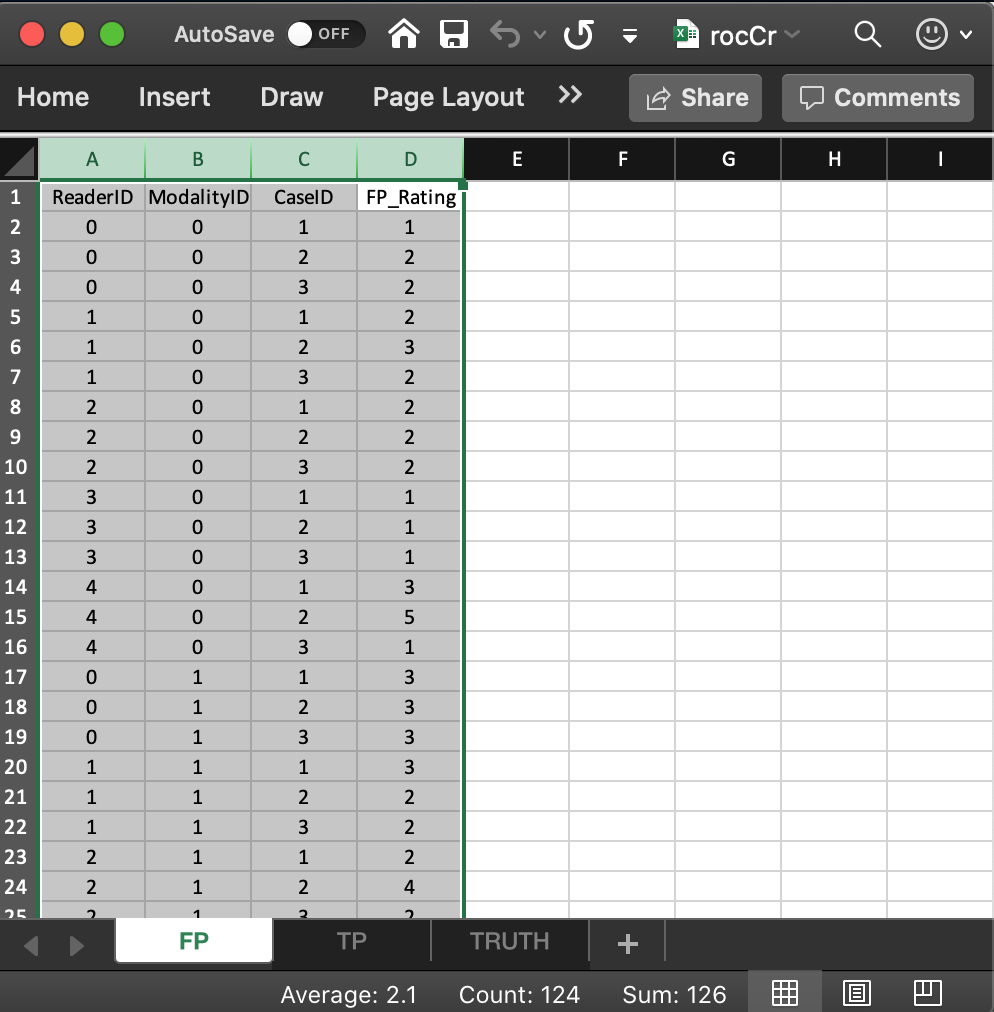
\includegraphics[width=0.5\linewidth,height=0.2\textheight]{images/rocCrFp} 

}

\caption{FP worksheet for file rocCr.xlsx}\label{fig:showRocCrFpSheet}
\end{figure}

\begin{itemize}
\tightlist
\item
  It consists of 4 columns, each of length 30 (= \# of modalities times number of readers times number of non-diseased cases).
\item
  \texttt{ReaderID}: the reader labels: \texttt{0}, \texttt{1}, \texttt{2}, \texttt{3} and \texttt{4}. Each reader label occurs 6 times (= \# of modalities times number of non-diseased cases).
\item
  \texttt{ModalityID}: the modality or treatment labels: \texttt{0} and \texttt{1}. Each label occurs 15 times (= \# of readers times number of non-diseased cases).
\item
  \texttt{CaseID}: the case labels for non-diseased cases: \texttt{1}, \texttt{2} and \texttt{3}. Each label occurs 10 times (= \# of modalities times \# of readers).
\item
  The label of a diseased case cannot occur in the FP worksheet. If it does the software generates an error.
\item
  \texttt{FP\_Rating}: the floating point ratings of non-diseased cases. Each row of this worksheet contains a rating corresponding to the values of \texttt{ReaderID}, \texttt{ModalityID} and \texttt{CaseID} for that row.
\end{itemize}

\hypertarget{the-true-positive-tp-ratings}{%
\section{The true positive (TP) ratings}\label{the-true-positive-tp-ratings}}

These are found in the \texttt{TP} or \texttt{LL} worksheet, see below.

\begin{figure}

{\centering 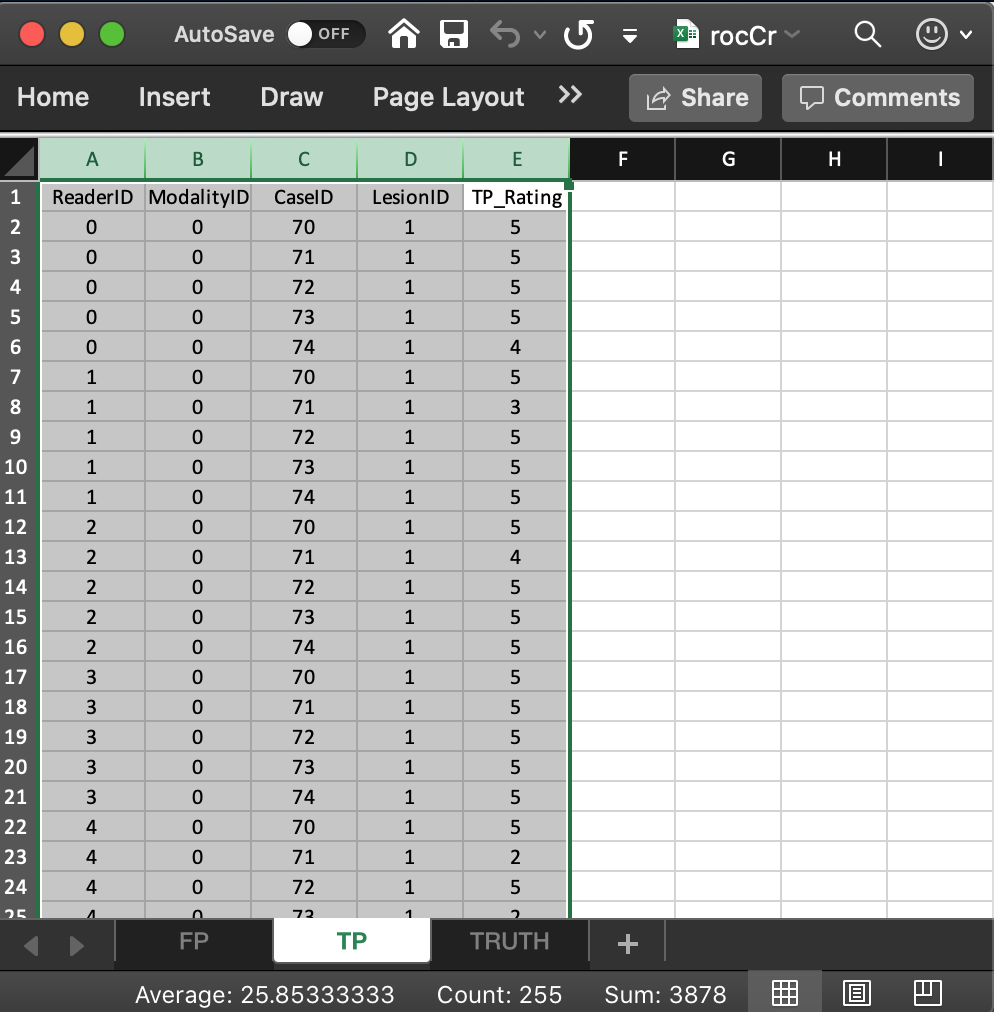
\includegraphics[width=0.5\linewidth,height=0.2\textheight]{images/rocCrTp} 

}

\caption{TP worksheet for file rocCr.xlsx}\label{fig:showRocCrTpSheet}
\end{figure}

\begin{itemize}
\tightlist
\item
  It consists of 5 columns, each of length 50 (= \# of modalities times number of readers times number of diseased cases).
\item
  \texttt{ReaderID}: the reader labels: \texttt{0}, \texttt{1}, \texttt{2}, \texttt{3} and \texttt{4}. Each reader label occurs 10 times (= \# of modalities times number of diseased cases).
\item
  \texttt{ModalityID}: the modality or treatment labels: \texttt{0} and \texttt{1}. Each label occurs 25 times (= \# of readers times number of diseased cases).
\item
  \texttt{LesionID}: For an ROC dataset this column contains fifty 1's (each diseased case has one lesion).
\item
  \texttt{CaseID}: the case labels for non-diseased cases: \texttt{70}, \texttt{71}, \texttt{72}, \texttt{73} and \texttt{74}. Each label occurs 10 times (= \# of modalities times \# of readers). The label of a non-diseased case cannot occur in the TP worksheet.
\item
  \texttt{TP\_Rating}: the floating point ratings of diseased cases. Each row of this worksheet contains a rating corresponding to the values of \texttt{ReaderID}, \texttt{ModalityID}, \texttt{LesionID} and \texttt{CaseID} for that row.
\end{itemize}

\hypertarget{correspondence-between-nl-member-of-dataset-and-the-fp-worksheet}{%
\section{\texorpdfstring{Correspondence between \texttt{NL} member of dataset and the \texttt{FP} worksheet}{Correspondence between NL member of dataset and the FP worksheet}}\label{correspondence-between-nl-member-of-dataset-and-the-fp-worksheet}}

\begin{itemize}
\tightlist
\item
  The list member \texttt{x\$NL} is an array with \texttt{dim\ =\ c(2,5,8,1)}.

  \begin{itemize}
  \tightlist
  \item
    The first dimension (2) comes from the number of modalities.
  \item
    The second dimension (5) comes from the number of readers.
  \item
    The third dimension (8) comes from the \textbf{total} number of cases.
  \item
    The fourth dimension is alway 1 for an ROC dataset.
  \end{itemize}
\item
  The value of \texttt{x\$NL{[}1,5,2,1{]}}, i.e., 5, corresponds to row 15 of the FP table, i.e., to \texttt{ModalityID} = 0, \texttt{ReaderID} = 4 and \texttt{CaseID} = 2.
\item
  The value of \texttt{x\$NL{[}2,3,2,1{]}}, i.e., 4, corresponds to row 24 of the FP table, i.e., to \texttt{ModalityID} 1, \texttt{ReaderID} 2 and \texttt{CaseID} 2.
\item
  All values for case index \textgreater{} 3 are \texttt{-Inf}. For example the value of \texttt{x\$NL{[}2,3,4,1{]}} is \texttt{-Inf}. This is because there are only 3 non-diseased cases. The extra length is needed for compatibility with FROC datasets.
\end{itemize}

\hypertarget{correspondence-between-ll-member-of-dataset-and-the-tp-worksheet}{%
\section{\texorpdfstring{Correspondence between \texttt{LL} member of dataset and the \texttt{TP} worksheet}{Correspondence between LL member of dataset and the TP worksheet}}\label{correspondence-between-ll-member-of-dataset-and-the-tp-worksheet}}

\begin{itemize}
\tightlist
\item
  The list member \texttt{x\$LL} is an array with \texttt{dim\ =\ c(2,5,5,1)}.

  \begin{itemize}
  \tightlist
  \item
    The first dimension (2) comes from the number of modalities.
  \item
    The second dimension (5) comes from the number of readers.
  \item
    The third dimension (5) comes from the number of diseased cases.
  \item
    The fourth dimension is alway 1 for an ROC dataset.
  \end{itemize}
\item
  The value of \texttt{x\$LL{[}1,1,5,1{]}}, i.e., 4, corresponds to row 6 of the TP table, i.e., to \texttt{ModalityID} = 0, \texttt{ReaderID} = 0 and \texttt{CaseID} = 74.
\item
  The value of \texttt{x\$LL{[}1,2,2,1{]}}, i.e., 3, corresponds to row 8 of the TP table, i.e., to \texttt{ModalityID} = 0, \texttt{ReaderID} = 1 and \texttt{CaseID} = 71.
\item
  There are no -Inf values in \texttt{x\$LL}: \texttt{any(x\$LL\ ==\ -Inf)} = FALSE.
\end{itemize}

\hypertarget{correspondence-using-the-which-function}{%
\section{\texorpdfstring{Correspondence using the \texttt{which} function}{Correspondence using the which function}}\label{correspondence-using-the-which-function}}

\begin{itemize}
\tightlist
\item
  Converting from \textbf{names} to \textbf{subscripts} (indicating position in an array) can be confusing.
\item
  The following example uses the \texttt{which} function to help out.
\item
  The first line says that the \texttt{abnormalCase} named 70 corresponds to subscript 1 in the LL array case dimension.
\item
  The second line prints the NL rating for \texttt{modalityID} = 0, \texttt{readerID} = 1 and \texttt{normalCases} = 1.
\item
  The third line prints the LL rating for \texttt{modalityID} = 0, \texttt{readerID} = 1 and \texttt{abnormalCases} = 70.
\item
  The last line shows what happens if one enters an invalid value for name; the result is a \texttt{numeric(0)}.
\item
  Note that in each of these examples, the last dimension is 1 because we are dealing with an ROC dataset.
\item
  The reader is encouraged to examine the correspondence between the NL and LL ratings and the Excel file using this method.
\end{itemize}

\begin{Shaded}
\begin{Highlighting}[]
\KeywordTok{which}\NormalTok{(x}\OperatorTok{$}\NormalTok{abnormalCases }\OperatorTok{==}\StringTok{ }\DecValTok{70}\NormalTok{)}
\CommentTok{#> [1] 1}
\NormalTok{x}\OperatorTok{$}\NormalTok{NL[}\KeywordTok{which}\NormalTok{(x}\OperatorTok{$}\NormalTok{modalityID }\OperatorTok{==}\StringTok{ "0"}\NormalTok{),}\KeywordTok{which}\NormalTok{(x}\OperatorTok{$}\NormalTok{readerID }\OperatorTok{==}\StringTok{ "1"}\NormalTok{),}\KeywordTok{which}\NormalTok{(x}\OperatorTok{$}\NormalTok{normalCases }\OperatorTok{==}\StringTok{ }\DecValTok{1}\NormalTok{),}\DecValTok{1}\NormalTok{]}
\CommentTok{#> [1] 2}
\NormalTok{x}\OperatorTok{$}\NormalTok{LL[}\KeywordTok{which}\NormalTok{(x}\OperatorTok{$}\NormalTok{modalityID }\OperatorTok{==}\StringTok{ "0"}\NormalTok{),}\KeywordTok{which}\NormalTok{(x}\OperatorTok{$}\NormalTok{readerID }\OperatorTok{==}\StringTok{ "1"}\NormalTok{),}\KeywordTok{which}\NormalTok{(x}\OperatorTok{$}\NormalTok{abnormalCases }\OperatorTok{==}\StringTok{ }\DecValTok{70}\NormalTok{),}\DecValTok{1}\NormalTok{]}
\CommentTok{#> [1] 5}
\NormalTok{x}\OperatorTok{$}\NormalTok{LL[}\KeywordTok{which}\NormalTok{(x}\OperatorTok{$}\NormalTok{modalityID }\OperatorTok{==}\StringTok{ "a"}\NormalTok{),}\KeywordTok{which}\NormalTok{(x}\OperatorTok{$}\NormalTok{readerID }\OperatorTok{==}\StringTok{ "1"}\NormalTok{),}\KeywordTok{which}\NormalTok{(x}\OperatorTok{$}\NormalTok{abnormalCases }\OperatorTok{==}\StringTok{ }\DecValTok{70}\NormalTok{),}\DecValTok{1}\NormalTok{]}
\CommentTok{#> numeric(0)}
\end{Highlighting}
\end{Shaded}

\hypertarget{frocdataformat}{%
\chapter{FROC data format}\label{frocdataformat}}

\hypertarget{purpose}{%
\section{Purpose}\label{purpose}}

\begin{itemize}
\tightlist
\item
  Explain the data format of the input Excel file for FROC datasets.
\item
  Explain the format of the FROC dataset.
\item
  Explain the lesion distribution array returned by \texttt{UtilLesionDistr()}.
\item
  Explain the lesion weights array returned by \texttt{UtilLesionWeightsDistr()}.
\item
  Details on the FROC paradigm are in my book.
\end{itemize}

\hypertarget{introduction-1}{%
\section{Introduction}\label{introduction-1}}

\begin{itemize}
\tightlist
\item
  See my book \citet{RN2680} for full details.
\item
  In the Free-response Receiver Operating Characteristic (FROC) paradigm \citep{RN761} the observer searches each case for signs of \textbf{localized disease} and marks and rates localized regions that are sufficiently suspicious for disease presence.
\item
  FROC data consists of \textbf{mark-rating pairs}, where each mark is a localized-region that was considered sufficiently suspicious for presence of a localized lesion and the rating is the corresponding confidence level.
\item
  By adopting a proximity criterion, each mark is classified by the investigator as a lesion localization (\texttt{LL}) - if it is close to a real lesion - or a non-lesion localization (\texttt{NL}) otherwise.
\item
  The observer assigns a rating to each region. The rating, as in the ROC paradigm, can be an integer or quasi-continuous (e.g., 0 -- 100), or a floating point value, as long as higher numbers represent greater confidence in presence of a lesion at the indicated region.
\end{itemize}

\hypertarget{the-excel-data-format-1}{%
\section{The Excel data format}\label{the-excel-data-format-1}}

The Excel file has three worsheets. These are named \texttt{Truth}, \texttt{NL} or \texttt{FP} and \texttt{LL} or \texttt{TP}.

\hypertarget{the-truth-worksheet-1}{%
\section{\texorpdfstring{The \texttt{Truth} worksheet}{The Truth worksheet}}\label{the-truth-worksheet-1}}

The \texttt{Truth} worksheet contains 6 columns: \texttt{CaseID}, \texttt{LesionID}, \texttt{Weight}, \texttt{ReaderID}, \texttt{ModalityID} and \texttt{Paradigm}.

\begin{itemize}
\tightlist
\item
  Since a diseased case may have more than one lesion, the first five columns contain \textbf{at least} as many rows as there are cases (images) in the dataset.
\item
  \texttt{CaseID}: unique \textbf{integers}, one per case, representing the cases in the dataset.
\item
  \texttt{LesionID}: integers 0, 1, 2, etc., with each 0 representing a non-diseased case, 1 representing the \emph{first} lesion on a diseased case, 2 representing the second lesion on a diseased case, if present, and so on.
\item
  The non-diseased cases are labeled \texttt{1}, \texttt{2} and \texttt{3}, while the diseased cases are labeled \texttt{70}, \texttt{71}, \texttt{72}, \texttt{73} and \texttt{74}.
\item
  There are 3 non-diseased cases in the dataset (the number of 0's in the \texttt{LesionID} column).
\item
  There are 5 diseased cases in the dataset (the number of 1's in the \texttt{LesionID} column of the \texttt{Truth} worksheet).
\item
  There are 3 readers in the dataset (each cell in the \texttt{ReaderID} column contains \texttt{0,\ 1,\ 2}).
\item
  There are 2 modalities in the dataset (each cell in the \texttt{ModalityID} column contains \texttt{0,\ 1}).
\item
  \texttt{Weight}: floating point; 0, for each non-diseased case, or values for each diseased case that add up to unity.\\
\item
  Diseased case \texttt{70} has two lesions, with \texttt{LesionID}s 1 and 2, and weights 0.3 and 0.7. Diseased case \texttt{71} has one lesion, with \texttt{LesionID} = 1, and \texttt{Weight} = 1. Diseased case \texttt{72} has three lesions, with \texttt{LesionID}s 1, 2 and 3 and weights 1/3 each. Diseased case \texttt{73} has two lesions, with \texttt{LesionID}s 1, and 2 and weights 0.1 and 0.9. Diseased case \texttt{74} has one lesion, with \texttt{LesionID} = 1 and \texttt{Weight} = 1.
\item
  \texttt{ReaderID}: a comma-separated listing of readers, each represented by a unique \textbf{integer}, that have interpreted the case. In the example shown below each cell has the value \texttt{0,\ 1,\ 2}. \textbf{Each cell has to be text formatted. Otherwise Excel will not accept it.}
\item
  \texttt{ModalityID}: a comma-separated listing of modalities (or treatments), each represented by a unique \textbf{integer}, that apply to each case. In the example each cell has the value \texttt{0,\ 1}. \textbf{Each cell has to be text formatted.}
\item
  \texttt{Paradigm}: In the example shown below, the contents are \texttt{FROC} and \texttt{crossed}. It informs the software that this is an \texttt{FROC} dataset and the design is ``crossed'', as in \textbf{Vignette \#1}.
\end{itemize}

\begin{figure}

{\centering 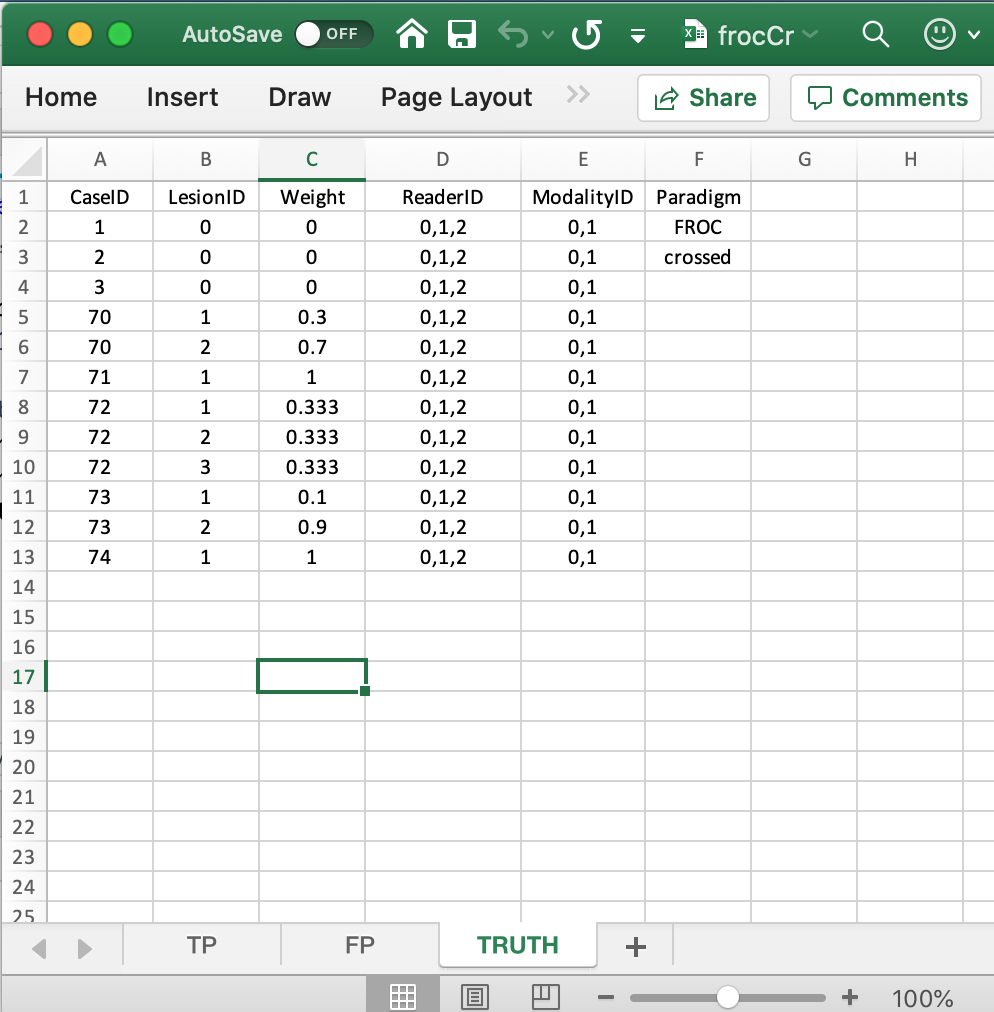
\includegraphics[width=0.5\linewidth,height=0.2\textheight]{images/frocCrTruth} 

}

\caption{Truth worksheet for file inst/extdata/toyFiles/FROC/frocCr.xlsx}\label{fig:frocCrTruth}
\end{figure}

\hypertarget{the-structure-of-an-froc-dataset}{%
\section{The structure of an FROC dataset}\label{the-structure-of-an-froc-dataset}}

The example shown above corresponds to Excel file \texttt{inst/extdata/toyFiles/FROC/frocCr.xlsx} in the project directory.

\begin{Shaded}
\begin{Highlighting}[]
\NormalTok{frocCr <-}\StringTok{ }\KeywordTok{system.file}\NormalTok{(}\StringTok{"extdata"}\NormalTok{, }\StringTok{"toyFiles/FROC/frocCr.xlsx"}\NormalTok{,}
                        \DataTypeTok{package =} \StringTok{"RJafroc"}\NormalTok{, }\DataTypeTok{mustWork =} \OtherTok{TRUE}\NormalTok{)}
\NormalTok{x <-}\StringTok{ }\KeywordTok{DfReadDataFile}\NormalTok{(frocCr, }\DataTypeTok{newExcelFileFormat =} \OtherTok{TRUE}\NormalTok{)}
\KeywordTok{str}\NormalTok{(x)}
\CommentTok{#> List of 12}
\CommentTok{#>  $ NL           : num [1:2, 1:3, 1:8, 1:2] 1.02 2.89 2.21 3.01 2.14 ...}
\CommentTok{#>  $ LL           : num [1:2, 1:3, 1:5, 1:3] 5.28 5.2 5.14 4.77 4.66 4.87 3.01 3.27 3.31 3.19 ...}
\CommentTok{#>  $ lesionVector : int [1:5] 2 1 3 2 1}
\CommentTok{#>  $ lesionID     : num [1:5, 1:3] 1 1 1 1 1 ...}
\CommentTok{#>  $ lesionWeight : num [1:5, 1:3] 0.3 1 0.333 0.1 1 ...}
\CommentTok{#>  $ dataType     : chr "FROC"}
\CommentTok{#>  $ modalityID   : Named chr [1:2] "0" "1"}
\CommentTok{#>   ..- attr(*, "names")= chr [1:2] "0" "1"}
\CommentTok{#>  $ readerID     : Named chr [1:3] "0" "1" "2"}
\CommentTok{#>   ..- attr(*, "names")= chr [1:3] "0" "1" "2"}
\CommentTok{#>  $ design       : chr "CROSSED"}
\CommentTok{#>  $ normalCases  : int [1:3] 1 2 3}
\CommentTok{#>  $ abnormalCases: int [1:5] 70 71 72 73 74}
\CommentTok{#>  $ truthTableStr: num [1:2, 1:3, 1:8, 1:4] 1 1 1 1 1 1 1 1 1 1 ...}
\end{Highlighting}
\end{Shaded}

\begin{itemize}
\tightlist
\item
  This follows the general description in \textbf{Vignette \#1}. The differences are described below.
\item
  The \texttt{x\$dataType} member indicates that this is an \texttt{FROC} dataset.
\item
  The \texttt{x\$lesionVector} member is a vector whose contents reflect the number of lesions in each diseased case, i.e., 2, 1, 3, 2, 1 in the current example.
\item
  The \texttt{x\$lesionID} member indicates the labeling of the lesions in each diseased case.
\end{itemize}

\begin{Shaded}
\begin{Highlighting}[]
\NormalTok{x}\OperatorTok{$}\NormalTok{lesionID}
\CommentTok{#>      [,1] [,2] [,3]}
\CommentTok{#> [1,]    1    2 -Inf}
\CommentTok{#> [2,]    1 -Inf -Inf}
\CommentTok{#> [3,]    1    2    3}
\CommentTok{#> [4,]    1    2 -Inf}
\CommentTok{#> [5,]    1 -Inf -Inf}
\end{Highlighting}
\end{Shaded}

\begin{itemize}
\tightlist
\item
  This shows that the lesions on the first diseased case are labeled 1 and 2. The \texttt{-Inf} is a filler used to denote a missing value. The second diseased case has one lesion labeled 1. The third diseased case has three lesions labeled 1, 2 and 3, etc.
\item
  The \texttt{lesionWeight} member is the clinical importance of each lesion. Lacking specific clinical reasons, the lesions should be equally weighted; this is \emph{not} true for this toy dataset.
\end{itemize}

\begin{Shaded}
\begin{Highlighting}[]
\NormalTok{x}\OperatorTok{$}\NormalTok{lesionWeight}
\CommentTok{#>           [,1]      [,2]      [,3]}
\CommentTok{#> [1,] 0.3000000 0.7000000      -Inf}
\CommentTok{#> [2,] 1.0000000      -Inf      -Inf}
\CommentTok{#> [3,] 0.3333333 0.3333333 0.3333333}
\CommentTok{#> [4,] 0.1000000 0.9000000      -Inf}
\CommentTok{#> [5,] 1.0000000      -Inf      -Inf}
\end{Highlighting}
\end{Shaded}

\begin{itemize}
\tightlist
\item
  The first diseased case has two lesions, the first has weight 0.3 and the second has weight 0.7. The second diseased case has one lesion with weight 1.The third diseased case has three equally weighted lesions, each with weight 1/3. Etc.
\end{itemize}

\hypertarget{the-false-positive-fp-ratings-1}{%
\section{The false positive (FP) ratings}\label{the-false-positive-fp-ratings-1}}

These are found in the \texttt{FP} or \texttt{NL} worksheet, see below.

\begin{figure}

{\centering 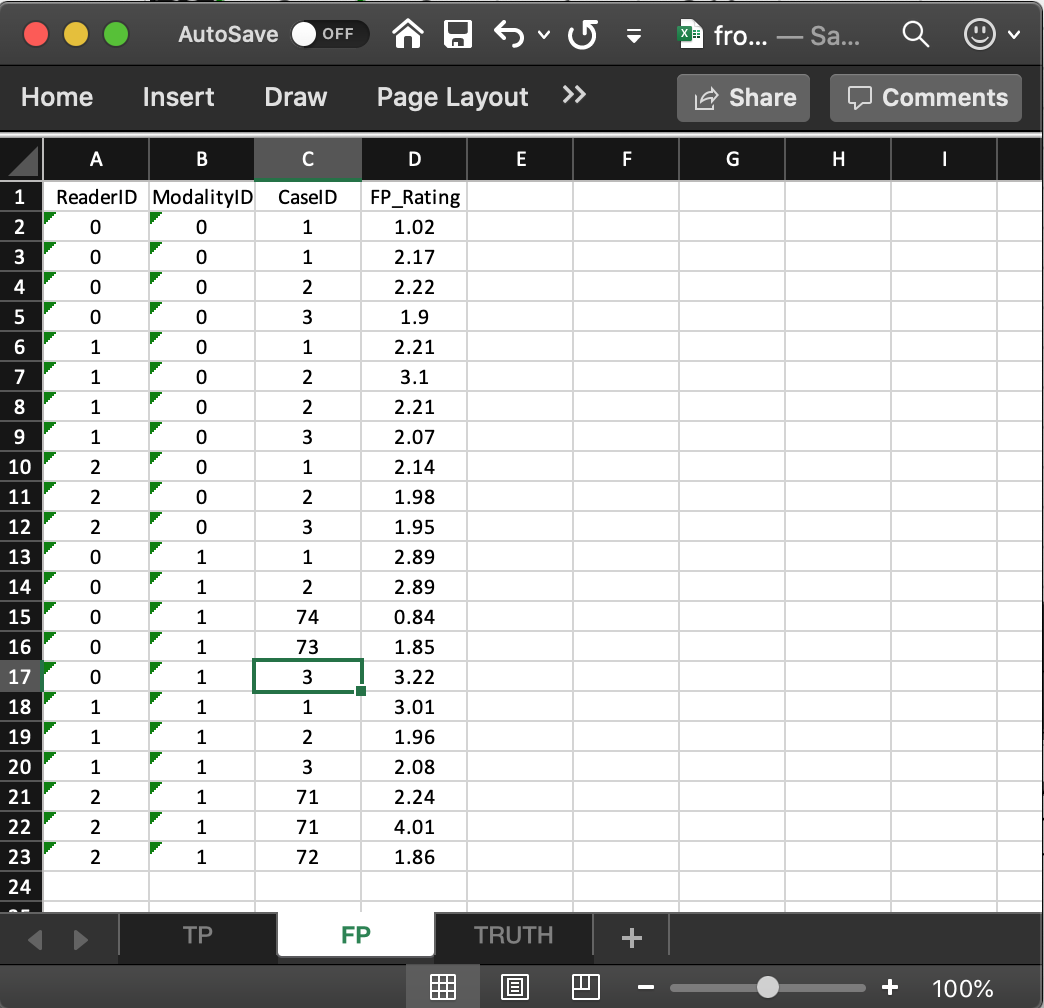
\includegraphics[width=0.5\linewidth,height=0.2\textheight]{images/frocCrNL} 

}

\caption{Fig. 2: FP/NL worksheet for file inst/extdata/toyFiles/FROC/frocCr.xlsx}\label{fig:frocCrNL}
\end{figure}

\begin{itemize}
\tightlist
\item
  It consists of 4 columns, of equal length. \textbf{The common length is unpredictable.} It could be zero if the dataset has no NL marks (a distinct possibility if the lesions are very easy to find and the modality and/or observer has high performance). All one knows is that the common length is an integer greater than or equal to zero.
\item
  In the example dataset, the common length is 22.
\item
  \texttt{ReaderID}: the reader labels: these must be \texttt{0}, \texttt{1}, or \texttt{2}, as declared in the \texttt{Truth} worksheet.
\item
  \texttt{ModalityID}: the modality labels: must be \texttt{0} or \texttt{1}, as declared in the \texttt{Truth} worksheet.
\item
  \texttt{CaseID}: the labels of cases with \texttt{NL} marks. In the FROC paradigm, \texttt{NL} events can occur on non-diseased \textbf{and} diseased cases.
\item
  \texttt{FP\_Rating}: the floating point ratings of \texttt{NL} marks. Each row of this worksheet yields a rating corresponding to the values of \texttt{ReaderID}, \texttt{ModalityID} and \texttt{CaseID} for that row.
\item
  For \texttt{ModalityID} 0, \texttt{ReaderID} 0 and \texttt{CaseID} 1 (the first non-diseased case declared in the \texttt{Truth} worksheet), there is a single \texttt{NL} mark that was rated 1.02, corresponding to row 2 of the \texttt{FP} worksheet.
\item
  Diseased cases with \texttt{NL} marks are also declared in the \texttt{FP} worksheet. Some examples are seen at rows 15, 16 and 21-23 of the \texttt{FP} worksheet.
\item
  Rows 21 and 22 show that \texttt{caseID} = 71 got two \texttt{NL} marks, rated 2.24, 4.01.
\item
  That this is the \emph{only} case with two marks determines the length of the fourth dimension of the \texttt{x\$NL} list member, 2 in the current example. Absent this case, the length would have been one.
\item
  In general, the case with the most \texttt{NL} marks determines the length of the fourth dimension of the \texttt{x\$NL} list member.
\item
  The reader should convince oneself that the ratings in \texttt{x\$NL} reflect the contents of the \texttt{FP} worksheet.
\end{itemize}

\hypertarget{the-true-positive-tp-ratings-1}{%
\section{The true positive (TP) ratings}\label{the-true-positive-tp-ratings-1}}

These are found in the \texttt{TP} or \texttt{LL} worksheet, see below.

\begin{figure}

{\centering 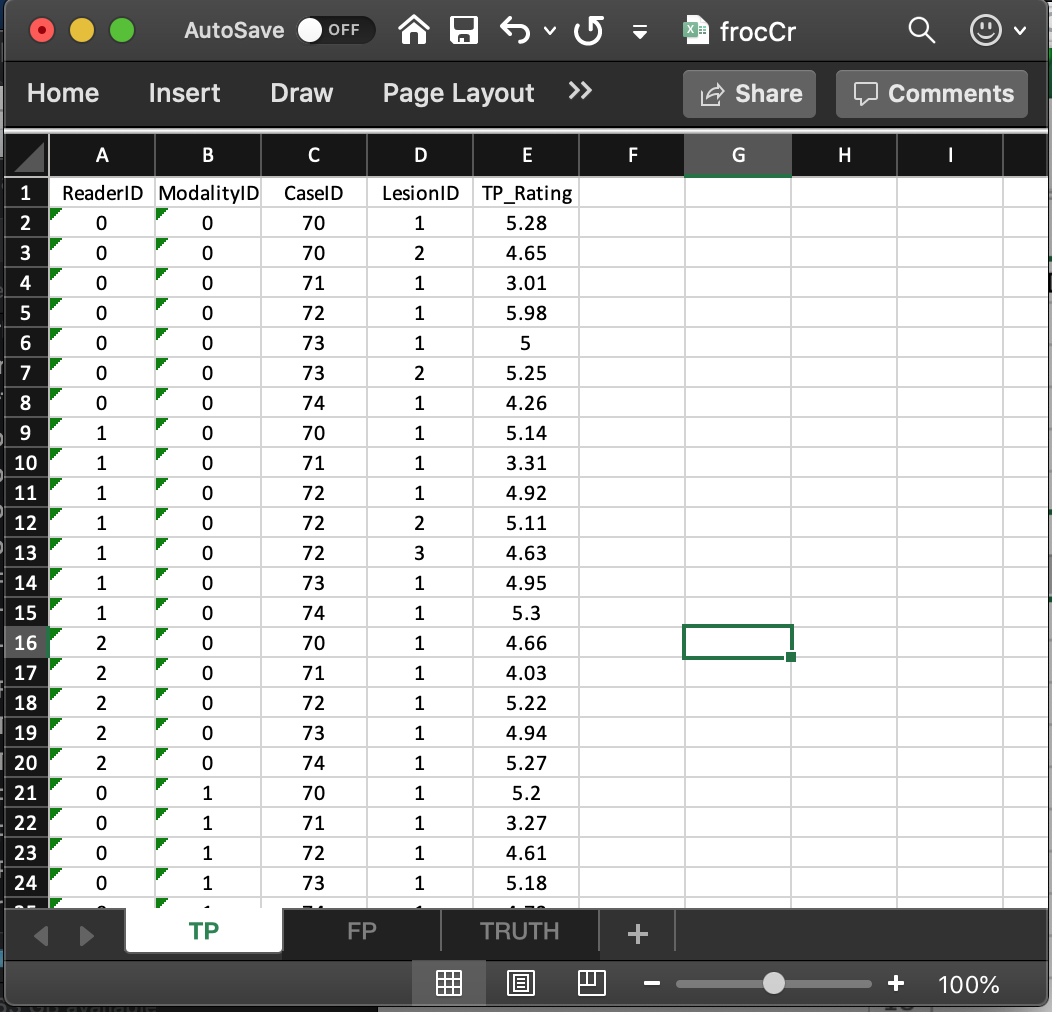
\includegraphics[width=0.5\linewidth,height=0.2\textheight]{images/frocCrLL} 

}

\caption{Fig. 3: TP/LL worksheet for file inst/extdata/toyFiles/FROC/frocCr.xlsx}\label{fig:frocCrLL}
\end{figure}

\begin{itemize}
\tightlist
\item
  This worksheet can only have diseased cases. The presence of a non-diseased case in this worksheet will generate an error.
\item
  The common vertical length, 31 in this example, is a-priori unpredictable. Given the structure of the \texttt{Truth} worsheet for this dataset, the maximum length would be 9 times 2 times 3, assuming every lesion is marked for each modality, reader and diseased case. The 9 comes from the total number of non-zero entries in the \texttt{LesionID} column of the \texttt{Truth} worksheet.
\item
  The fact that the length is smaller than the maximum length means that there are combinations of modality, reader and diseased cases on which some lesions were not marked.
\item
  As an example, the first lesion in \texttt{CaseID} equal to \texttt{70} was marked (and rated 5.28) in \texttt{ModalityID} \texttt{0} and \texttt{ReaderID} \texttt{0}.
\item
  The length of the fourth dimension of the \texttt{x\$LL} list member, 3 in the present example, is determined by the diseased case with the most lesions in the \texttt{Truth} worksheet.
\item
  The reader should convince oneself that the ratings in \texttt{x\$LL} reflect the contents of the \texttt{TP} worksheet.
\end{itemize}

\hypertarget{on-the-distribution-of-numbers-of-lesions-in-abnormal-cases}{%
\section{On the distribution of numbers of lesions in abnormal cases}\label{on-the-distribution-of-numbers-of-lesions-in-abnormal-cases}}

\begin{itemize}
\tightlist
\item
  Consider a much larger dataset, \texttt{dataset11}, with structure as shown below:
\end{itemize}

\begin{Shaded}
\begin{Highlighting}[]
\NormalTok{x <-}\StringTok{ }\NormalTok{dataset11}
\KeywordTok{str}\NormalTok{(x)}
\CommentTok{#> List of 12}
\CommentTok{#>  $ NL           : num [1:4, 1:5, 1:158, 1:4] -Inf -Inf -Inf -Inf -Inf ...}
\CommentTok{#>  $ LL           : num [1:4, 1:5, 1:115, 1:20] -Inf -Inf -Inf -Inf -Inf ...}
\CommentTok{#>  $ lesionVector : int [1:115] 6 4 7 1 3 3 3 8 11 2 ...}
\CommentTok{#>  $ lesionID     : num [1:115, 1:20] 1 1 1 1 1 1 1 1 1 1 ...}
\CommentTok{#>  $ lesionWeight : num [1:115, 1:20] 0.167 0.25 0.143 1 0.333 ...}
\CommentTok{#>  $ dataType     : chr "FROC"}
\CommentTok{#>  $ modalityID   : Named chr [1:4] "1" "2" "3" "4"}
\CommentTok{#>   ..- attr(*, "names")= chr [1:4] "1" "2" "3" "4"}
\CommentTok{#>  $ readerID     : Named chr [1:5] "1" "2" "3" "4" ...}
\CommentTok{#>   ..- attr(*, "names")= chr [1:5] "1" "2" "3" "4" ...}
\CommentTok{#>  $ design       : chr "CROSSED"}
\CommentTok{#>  $ normalCases  : int [1:43] 6 9 14 27 62 66 70 71 83 91 ...}
\CommentTok{#>  $ abnormalCases: int [1:115] 1 2 3 5 7 8 10 11 13 17 ...}
\CommentTok{#>  $ truthTableStr: num [1:4, 1:5, 1:158, 1:21] 1 1 1 1 1 1 1 1 1 1 ...}
\end{Highlighting}
\end{Shaded}

\begin{itemize}
\tightlist
\item
  Focus for now in the 115 abnormal cases.
\item
  The numbers of lesions in these cases is contained in \texttt{x\$lesionVector}.
\end{itemize}

\begin{Shaded}
\begin{Highlighting}[]
\NormalTok{x}\OperatorTok{$}\NormalTok{lesionVector}
\CommentTok{#>   [1]  6  4  7  1  3  3  3  8 11  2  4  6  2 16  5  2  8  3  4  7 11  1  4  3  4}
\CommentTok{#>  [26]  4  7  3  2  5  2  2  7  6  6  4 10 20 12  6  4  7 12  5  1  1  5  1  2  8}
\CommentTok{#>  [51]  3  1  2  2  3  2  8 16 10  1  2  2  6  3  2  2  4  6 10 11  1  2  6  2  4}
\CommentTok{#>  [76]  5  2  9  6  6  8  3  8  7  1  1  6  3  2  1  9  8  8  2  2 12  1  1  1  1}
\CommentTok{#> [101]  1  3  1  2  2  1  1  1  1  3  1  1  1  2  1}
\end{Highlighting}
\end{Shaded}

\begin{itemize}
\tightlist
\item
  For example, the first abnormal case contains 6 lesions, the second contains 4 lesions, the third contains 7 lesions, etc. and the last abnormal case contains 1 lesion.
\item
  To get an idea of the distribution of the numbers of lesions per abnormal cases, one could interrogate this vector as shown below using the \texttt{which()} function:
\end{itemize}

\begin{Shaded}
\begin{Highlighting}[]
\ControlFlowTok{for}\NormalTok{ (el }\ControlFlowTok{in} \DecValTok{1}\OperatorTok{:}\KeywordTok{max}\NormalTok{(x}\OperatorTok{$}\NormalTok{lesionVector)) }\KeywordTok{cat}\NormalTok{(}
  \StringTok{"abnormal cases with"}\NormalTok{, el, }\StringTok{"lesions = "}\NormalTok{, }
  \KeywordTok{length}\NormalTok{(}\KeywordTok{which}\NormalTok{(x}\OperatorTok{$}\NormalTok{lesionVector }\OperatorTok{==}\StringTok{ }\NormalTok{el)), }\StringTok{"}\CharTok{\textbackslash{}n}\StringTok{"}\NormalTok{)}
\CommentTok{#> abnormal cases with 1 lesions =  25 }
\CommentTok{#> abnormal cases with 2 lesions =  23 }
\CommentTok{#> abnormal cases with 3 lesions =  13 }
\CommentTok{#> abnormal cases with 4 lesions =  10 }
\CommentTok{#> abnormal cases with 5 lesions =  5 }
\CommentTok{#> abnormal cases with 6 lesions =  11 }
\CommentTok{#> abnormal cases with 7 lesions =  6 }
\CommentTok{#> abnormal cases with 8 lesions =  8 }
\CommentTok{#> abnormal cases with 9 lesions =  2 }
\CommentTok{#> abnormal cases with 10 lesions =  3 }
\CommentTok{#> abnormal cases with 11 lesions =  3 }
\CommentTok{#> abnormal cases with 12 lesions =  3 }
\CommentTok{#> abnormal cases with 13 lesions =  0 }
\CommentTok{#> abnormal cases with 14 lesions =  0 }
\CommentTok{#> abnormal cases with 15 lesions =  0 }
\CommentTok{#> abnormal cases with 16 lesions =  2 }
\CommentTok{#> abnormal cases with 17 lesions =  0 }
\CommentTok{#> abnormal cases with 18 lesions =  0 }
\CommentTok{#> abnormal cases with 19 lesions =  0 }
\CommentTok{#> abnormal cases with 20 lesions =  1}
\end{Highlighting}
\end{Shaded}

\begin{itemize}
\tightlist
\item
  This tells us that 25 cases contain 1 lesion
\item
  Likewise, 23 cases contain 2 lesions
\item
  Etc.
\end{itemize}

\hypertarget{definition-of-lesdistr-array}{%
\subsection{\texorpdfstring{Definition of \texttt{lesDistr} array}{Definition of lesDistr array}}\label{definition-of-lesdistr-array}}

\begin{itemize}
\tightlist
\item
  Let us ask what is the fraction of (abnormal) cases with 1 lesion, 2 lesions etc.
\end{itemize}

\begin{Shaded}
\begin{Highlighting}[]
\ControlFlowTok{for}\NormalTok{ (el }\ControlFlowTok{in} \DecValTok{1}\OperatorTok{:}\KeywordTok{max}\NormalTok{(x}\OperatorTok{$}\NormalTok{lesionVector)) }\KeywordTok{cat}\NormalTok{(}\StringTok{"fraction of abnormal cases with"}\NormalTok{, el, }\StringTok{"lesions = "}\NormalTok{, }
                                              \KeywordTok{length}\NormalTok{(}\KeywordTok{which}\NormalTok{(x}\OperatorTok{$}\NormalTok{lesionVector }\OperatorTok{==}\StringTok{ }\NormalTok{el))}\OperatorTok{/}\KeywordTok{length}\NormalTok{(x}\OperatorTok{$}\NormalTok{LL[}\DecValTok{1}\NormalTok{,}\DecValTok{1}\NormalTok{,,}\DecValTok{1}\NormalTok{]), }\StringTok{"}\CharTok{\textbackslash{}n}\StringTok{"}\NormalTok{)}
\CommentTok{#> fraction of abnormal cases with 1 lesions =  0.2173913 }
\CommentTok{#> fraction of abnormal cases with 2 lesions =  0.2 }
\CommentTok{#> fraction of abnormal cases with 3 lesions =  0.1130435 }
\CommentTok{#> fraction of abnormal cases with 4 lesions =  0.08695652 }
\CommentTok{#> fraction of abnormal cases with 5 lesions =  0.04347826 }
\CommentTok{#> fraction of abnormal cases with 6 lesions =  0.09565217 }
\CommentTok{#> fraction of abnormal cases with 7 lesions =  0.05217391 }
\CommentTok{#> fraction of abnormal cases with 8 lesions =  0.06956522 }
\CommentTok{#> fraction of abnormal cases with 9 lesions =  0.0173913 }
\CommentTok{#> fraction of abnormal cases with 10 lesions =  0.02608696 }
\CommentTok{#> fraction of abnormal cases with 11 lesions =  0.02608696 }
\CommentTok{#> fraction of abnormal cases with 12 lesions =  0.02608696 }
\CommentTok{#> fraction of abnormal cases with 13 lesions =  0 }
\CommentTok{#> fraction of abnormal cases with 14 lesions =  0 }
\CommentTok{#> fraction of abnormal cases with 15 lesions =  0 }
\CommentTok{#> fraction of abnormal cases with 16 lesions =  0.0173913 }
\CommentTok{#> fraction of abnormal cases with 17 lesions =  0 }
\CommentTok{#> fraction of abnormal cases with 18 lesions =  0 }
\CommentTok{#> fraction of abnormal cases with 19 lesions =  0 }
\CommentTok{#> fraction of abnormal cases with 20 lesions =  0.008695652}
\end{Highlighting}
\end{Shaded}

\begin{itemize}
\tightlist
\item
  This tells us that fraction 0.217 of (abnormal) cases contain 1 lesion
\item
  And fraction 0.2 of (abnormal) cases contain 2 lesions
\item
  Etc.
\item
  This information is contained the the \texttt{lesDistr} array
\item
  It is coded in the \texttt{Utility} function \texttt{UtilLesionDistr()}
\end{itemize}

\begin{Shaded}
\begin{Highlighting}[]
\NormalTok{lesDistr <-}\StringTok{ }\KeywordTok{UtilLesionDistr}\NormalTok{(x)}
\NormalTok{lesDistr}
\CommentTok{#>       [,1]        [,2]}
\CommentTok{#>  [1,]    1 0.217391304}
\CommentTok{#>  [2,]    2 0.200000000}
\CommentTok{#>  [3,]    3 0.113043478}
\CommentTok{#>  [4,]    4 0.086956522}
\CommentTok{#>  [5,]    5 0.043478261}
\CommentTok{#>  [6,]    6 0.095652174}
\CommentTok{#>  [7,]    7 0.052173913}
\CommentTok{#>  [8,]    8 0.069565217}
\CommentTok{#>  [9,]    9 0.017391304}
\CommentTok{#> [10,]   10 0.026086957}
\CommentTok{#> [11,]   11 0.026086957}
\CommentTok{#> [12,]   12 0.026086957}
\CommentTok{#> [13,]   16 0.017391304}
\CommentTok{#> [14,]   20 0.008695652}
\end{Highlighting}
\end{Shaded}

\begin{itemize}
\tightlist
\item
  The \texttt{UtilLesionDistr()} function returns an array with two columns and number of rows equal to the number of distinct values of lesions per case.
\item
  The first column contains the number of distinct values of lesions per case, 14 in the current example.
\item
  The second column contains the fraction of diseased cases with the number of lesions indicated in the first column.
\item
  The second column must sum to unity
\end{itemize}

\begin{Shaded}
\begin{Highlighting}[]
\KeywordTok{sum}\NormalTok{(}\KeywordTok{UtilLesionDistr}\NormalTok{(x)[,}\DecValTok{2}\NormalTok{])}
\CommentTok{#> [1] 1}
\end{Highlighting}
\end{Shaded}

\begin{itemize}
\tightlist
\item
  The lesion distribution array will come in handy when it comes to predicting the operating characteristics from using the Radiological Search Model (RSM), as detailed in Chapter 17 of my book.
\end{itemize}

\hypertarget{definition-of-leswghtdistr-array}{%
\section{\texorpdfstring{Definition of \texttt{lesWghtDistr} array}{Definition of lesWghtDistr array}}\label{definition-of-leswghtdistr-array}}

\begin{itemize}
\tightlist
\item
  This is returned by \texttt{UtilLesionWeightsDistr()}.
\item
  This contains the same number of rows as \texttt{lesDistr}.
\item
  The number of columns is one plus the number of rows as \texttt{lesDistr}.
\item
  The first column contains the number of distinct values of lesions per case, 14 in the current example.
\item
  The second column contains the weights of cases with number of lesions per case corresponding to row 1.
\item
  The third column contains the weights of cases with number of lesions per case corresponding to row 2.
\item
  Etc.
\item
  Missing values are filled with \texttt{-Inf}.
\end{itemize}

\begin{Shaded}
\begin{Highlighting}[]
\NormalTok{lesWghtDistr <-}\StringTok{ }\KeywordTok{UtilLesionWeightsDistr}\NormalTok{(x)}
\KeywordTok{cat}\NormalTok{(}\StringTok{"dim(lesDistr) ="}\NormalTok{, }\KeywordTok{dim}\NormalTok{(lesDistr),}\StringTok{"}\CharTok{\textbackslash{}n}\StringTok{"}\NormalTok{)}
\CommentTok{#> dim(lesDistr) = 14 2}
\KeywordTok{cat}\NormalTok{(}\StringTok{"dim(lesWghtDistr) ="}\NormalTok{, }\KeywordTok{dim}\NormalTok{(lesWghtDistr),}\StringTok{"}\CharTok{\textbackslash{}n}\StringTok{"}\NormalTok{)}
\CommentTok{#> dim(lesWghtDistr) = 14 21}
\KeywordTok{cat}\NormalTok{(}\StringTok{"lesWghtDistr = }\CharTok{\textbackslash{}n\textbackslash{}n}\StringTok{"}\NormalTok{)}
\CommentTok{#> lesWghtDistr =}
\NormalTok{lesWghtDistr}
\CommentTok{#>       [,1]       [,2]       [,3]       [,4]       [,5]       [,6]       [,7]}
\CommentTok{#>  [1,]    1 1.00000000       -Inf       -Inf       -Inf       -Inf       -Inf}
\CommentTok{#>  [2,]    2 0.50000000 0.50000000       -Inf       -Inf       -Inf       -Inf}
\CommentTok{#>  [3,]    3 0.33333333 0.33333333 0.33333333       -Inf       -Inf       -Inf}
\CommentTok{#>  [4,]    4 0.25000000 0.25000000 0.25000000 0.25000000       -Inf       -Inf}
\CommentTok{#>  [5,]    5 0.20000000 0.20000000 0.20000000 0.20000000 0.20000000       -Inf}
\CommentTok{#>  [6,]    6 0.16666667 0.16666667 0.16666667 0.16666667 0.16666667 0.16666667}
\CommentTok{#>  [7,]    7 0.14285714 0.14285714 0.14285714 0.14285714 0.14285714 0.14285714}
\CommentTok{#>  [8,]    8 0.12500000 0.12500000 0.12500000 0.12500000 0.12500000 0.12500000}
\CommentTok{#>  [9,]    9 0.11111111 0.11111111 0.11111111 0.11111111 0.11111111 0.11111111}
\CommentTok{#> [10,]   10 0.10000000 0.10000000 0.10000000 0.10000000 0.10000000 0.10000000}
\CommentTok{#> [11,]   11 0.09090909 0.09090909 0.09090909 0.09090909 0.09090909 0.09090909}
\CommentTok{#> [12,]   12 0.08333333 0.08333333 0.08333333 0.08333333 0.08333333 0.08333333}
\CommentTok{#> [13,]   16 0.06250000 0.06250000 0.06250000 0.06250000 0.06250000 0.06250000}
\CommentTok{#> [14,]   20 0.05000000 0.05000000 0.05000000 0.05000000 0.05000000 0.05000000}
\CommentTok{#>             [,8]       [,9]      [,10]      [,11]      [,12]      [,13]  [,14]}
\CommentTok{#>  [1,]       -Inf       -Inf       -Inf       -Inf       -Inf       -Inf   -Inf}
\CommentTok{#>  [2,]       -Inf       -Inf       -Inf       -Inf       -Inf       -Inf   -Inf}
\CommentTok{#>  [3,]       -Inf       -Inf       -Inf       -Inf       -Inf       -Inf   -Inf}
\CommentTok{#>  [4,]       -Inf       -Inf       -Inf       -Inf       -Inf       -Inf   -Inf}
\CommentTok{#>  [5,]       -Inf       -Inf       -Inf       -Inf       -Inf       -Inf   -Inf}
\CommentTok{#>  [6,]       -Inf       -Inf       -Inf       -Inf       -Inf       -Inf   -Inf}
\CommentTok{#>  [7,] 0.14285714       -Inf       -Inf       -Inf       -Inf       -Inf   -Inf}
\CommentTok{#>  [8,] 0.12500000 0.12500000       -Inf       -Inf       -Inf       -Inf   -Inf}
\CommentTok{#>  [9,] 0.11111111 0.11111111 0.11111111       -Inf       -Inf       -Inf   -Inf}
\CommentTok{#> [10,] 0.10000000 0.10000000 0.10000000 0.10000000       -Inf       -Inf   -Inf}
\CommentTok{#> [11,] 0.09090909 0.09090909 0.09090909 0.09090909 0.09090909       -Inf   -Inf}
\CommentTok{#> [12,] 0.08333333 0.08333333 0.08333333 0.08333333 0.08333333 0.08333333   -Inf}
\CommentTok{#> [13,] 0.06250000 0.06250000 0.06250000 0.06250000 0.06250000 0.06250000 0.0625}
\CommentTok{#> [14,] 0.05000000 0.05000000 0.05000000 0.05000000 0.05000000 0.05000000 0.0500}
\CommentTok{#>        [,15]  [,16]  [,17] [,18] [,19] [,20] [,21]}
\CommentTok{#>  [1,]   -Inf   -Inf   -Inf  -Inf  -Inf  -Inf  -Inf}
\CommentTok{#>  [2,]   -Inf   -Inf   -Inf  -Inf  -Inf  -Inf  -Inf}
\CommentTok{#>  [3,]   -Inf   -Inf   -Inf  -Inf  -Inf  -Inf  -Inf}
\CommentTok{#>  [4,]   -Inf   -Inf   -Inf  -Inf  -Inf  -Inf  -Inf}
\CommentTok{#>  [5,]   -Inf   -Inf   -Inf  -Inf  -Inf  -Inf  -Inf}
\CommentTok{#>  [6,]   -Inf   -Inf   -Inf  -Inf  -Inf  -Inf  -Inf}
\CommentTok{#>  [7,]   -Inf   -Inf   -Inf  -Inf  -Inf  -Inf  -Inf}
\CommentTok{#>  [8,]   -Inf   -Inf   -Inf  -Inf  -Inf  -Inf  -Inf}
\CommentTok{#>  [9,]   -Inf   -Inf   -Inf  -Inf  -Inf  -Inf  -Inf}
\CommentTok{#> [10,]   -Inf   -Inf   -Inf  -Inf  -Inf  -Inf  -Inf}
\CommentTok{#> [11,]   -Inf   -Inf   -Inf  -Inf  -Inf  -Inf  -Inf}
\CommentTok{#> [12,]   -Inf   -Inf   -Inf  -Inf  -Inf  -Inf  -Inf}
\CommentTok{#> [13,] 0.0625 0.0625 0.0625  -Inf  -Inf  -Inf  -Inf}
\CommentTok{#> [14,] 0.0500 0.0500 0.0500  0.05  0.05  0.05  0.05}
\end{Highlighting}
\end{Shaded}

\begin{itemize}
\tightlist
\item
  Row 3 corresponds to 3 lesions per case and the weights are 1/3, 1/3 and 1/3.
\item
  Row 13 corresponds to 16 lesions per case and the weights are 0.06250000, 0.06250000, \ldots{}, repeated 13 times.
\item
  Note that the number of rows is less than the maximum number of lesions per case (20).
\item
  This is because some configurations of lesions per case (e.g., cases with 13 lesions per case) do not occur in this dataset.
\end{itemize}

\hypertarget{summary}{%
\section{Summary}\label{summary}}

\begin{itemize}
\tightlist
\item
  The FROC dataset has far less regularity in structure as compared to an ROC dataset.
\item
  The length of the first dimension of either \texttt{x\$NL} or \texttt{x\$LL} list members is the total number of modalities, 2 in the current example.
\item
  The length of the second dimension of either \texttt{x\$NL} or \texttt{x\$LL} list members is the total number of readers, 3 in the current example.
\item
  The length of the third dimension of \texttt{x\$NL} is the total number of cases, 8 in the current example. The first three positions account for \texttt{NL} marks on non-diseased cases and the remaining 5 positions account for \texttt{NL} marks on diseased cases.
\item
  The length of the third dimension of \texttt{x\$LL} is the total number of diseased cases, 5 in the current example.
\item
  The length of the fourth dimension of \texttt{x\$NL} is determined by the case (diseased or non-diseased) with the most \texttt{NL} marks, 2 in the current example.
\item
  The length of the fourth dimension of \texttt{x\$LL} is determined by the diseased case with the most lesions, 3 in the current example.
\end{itemize}

\hypertarget{rocSpdataformat}{%
\chapter{ROC split plot data format}\label{rocSpdataformat}}

\hypertarget{introduction-2}{%
\section{Introduction}\label{introduction-2}}

\begin{itemize}
\tightlist
\item
  The purpose of this vignette is to explain the data format of the input Excel file for an ROC \emph{split-plot} dataset.
\item
  In a split-plot dataset each reader interprets a \emph{different} sub-set of cases in all modalities, i.e., the cases interpreted by different readers have no overlap.
\item
  Each sub-set of cases can have different numbers of non-diseased and diseased cases.
\item
  The example below assumes the same numbers of non-diseased and diseased cases.
\item
  The data format has been extended to \texttt{NewFormat} to allow such datasets.
\end{itemize}

\hypertarget{the-excel-data-format-2}{%
\section{The Excel data format}\label{the-excel-data-format-2}}

As before,the Excel file has three worsheets named \texttt{Truth}, \texttt{NL} or \texttt{FP} and \texttt{LL} or \texttt{TP}. The Excel file corresponding to the example that follows is \texttt{inst/extdata/toyFiles/ROC/rocSp.xlsx}.

\hypertarget{the-truth-worksheet-2}{%
\section{\texorpdfstring{The \texttt{Truth} worksheet}{The Truth worksheet}}\label{the-truth-worksheet-2}}

The \texttt{Truth} worksheet contains 6 columns: \texttt{CaseID}, \texttt{LesionID}, \texttt{Weight}, \texttt{ReaderID}, \texttt{ModalityID} and \texttt{Paradigm}.

\begin{itemize}
\tightlist
\item
  The first five columns contain as many rows as there are cases in the dataset.
\item
  \texttt{CaseID}: unique \textbf{integers}, one per case, representing the cases in the dataset.
\item
  \texttt{LesionID}: integers 0, representing non-diseased cases and 1 representing the diseased cases.
\item
  The \texttt{ReaderID} column is a listing of readers each represented by a \textbf{unique string}. Note that, unlike the crossed design, the \texttt{ReaderID} column has \emph{single values}. \textbf{Each cell has to be text formatted.}
\item
  The non-diseased cases interpreted by reader with \texttt{ReaderID} value \texttt{1} are labeled \texttt{6}, \texttt{7}, \texttt{8}, \texttt{9} and \texttt{10}, each with \texttt{LesionID} value \texttt{0}.
\item
  The diseased cases interpreted by this reader are labeled \texttt{16}, \texttt{17}, \texttt{18}, \texttt{19} and \texttt{20}, each with \texttt{LesionID} value \texttt{1}.\\
\item
  The second reader, with \texttt{ReaderID} value \texttt{4}, interprets five non-diseased cases labeled \texttt{21}, \texttt{22}, \texttt{23}, \texttt{24} and \texttt{25}, each with \texttt{LesionID} value \texttt{0}, and five diseased cases labeled \texttt{36}, \texttt{37}, \texttt{38}, \texttt{39} and \texttt{40}, each with \texttt{LesionID} value \texttt{1}.\\
\item
  The third reader, with ReaderID value \texttt{5}, interprets five non-diseased cases labeled \texttt{46}, \texttt{47}, \texttt{48}, \texttt{49} and \texttt{50}, each with \texttt{LesionID} value \texttt{0} and five diseased cases labeled \texttt{51}, \texttt{52}, \texttt{53}, \texttt{54} and \texttt{55}, each with \texttt{LesionID} value \texttt{1}.\\
\item
  \texttt{Weight}: floating point value 0 - this is not used for ROC data.\\
\item
  \texttt{ModalityID}: a comma-separated listing of modalities, each represented by a \textbf{unique string}. In the example shown below each cell has the value \texttt{1,\ 2}. \textbf{Each cell has to be text formatted.}
\item
  \texttt{Paradigm}: In the example shown in this vignette, the contents are \texttt{ROC} and \texttt{split-plot}.
\end{itemize}

\begin{figure}

{\centering 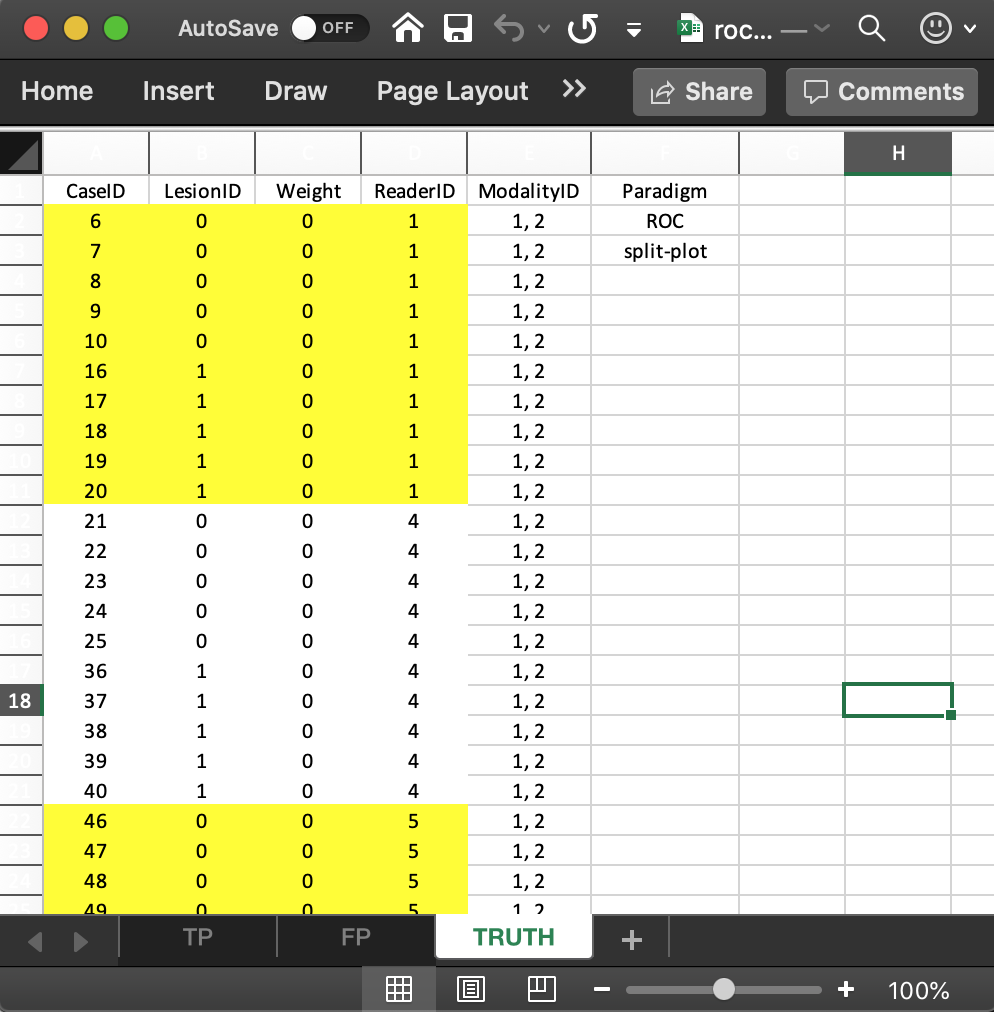
\includegraphics[width=0.5\linewidth,height=0.2\textheight]{images/rocSpTruth} 

}

\caption{Fig. 1: Truth worksheet for file inst/extdata/toyFiles/ROC/rocSp.xlsx}\label{fig:unnamed-chunk-1}
\end{figure}

\hypertarget{the-structure-of-the-roc-split-plot-dataset}{%
\section{The structure of the ROC split plot dataset}\label{the-structure-of-the-roc-split-plot-dataset}}

\begin{itemize}
\tightlist
\item
  The example shown in Fig. 1 corresponds to Excel file \texttt{inst/extdata/toyFiles/ROC/rocSp.xlsx} in the project directory.
\end{itemize}

\begin{Shaded}
\begin{Highlighting}[]
\NormalTok{rocSp <-}\StringTok{ }\KeywordTok{system.file}\NormalTok{(}\StringTok{"extdata"}\NormalTok{, }\StringTok{"toyFiles/ROC/rocSp.xlsx"}\NormalTok{,}
                        \DataTypeTok{package =} \StringTok{"RJafroc"}\NormalTok{, }\DataTypeTok{mustWork =} \OtherTok{TRUE}\NormalTok{)}
\NormalTok{x <-}\StringTok{ }\KeywordTok{DfReadDataFile}\NormalTok{(rocSp, }\DataTypeTok{newExcelFileFormat =} \OtherTok{TRUE}\NormalTok{)}
\KeywordTok{str}\NormalTok{(x)}
\CommentTok{#> List of 12}
\CommentTok{#>  $ NL           : num [1:2, 1:3, 1:30, 1] 1 1 -Inf -Inf -Inf ...}
\CommentTok{#>  $ LL           : num [1:2, 1:3, 1:15, 1] 5 2.3 -Inf -Inf -Inf ...}
\CommentTok{#>  $ lesionVector : int [1:15] 1 1 1 1 1 1 1 1 1 1 ...}
\CommentTok{#>  $ lesionID     : num [1:15, 1] 1 1 1 1 1 1 1 1 1 1 ...}
\CommentTok{#>  $ lesionWeight : num [1:15, 1] 1 1 1 1 1 1 1 1 1 1 ...}
\CommentTok{#>  $ dataType     : chr "ROC"}
\CommentTok{#>  $ modalityID   : Named chr [1:2] "1" "2"}
\CommentTok{#>   ..- attr(*, "names")= chr [1:2] "1" "2"}
\CommentTok{#>  $ readerID     : Named chr [1:3] "1" "4" "5"}
\CommentTok{#>   ..- attr(*, "names")= chr [1:3] "1" "4" "5"}
\CommentTok{#>  $ design       : chr "SPLIT-PLOT"}
\CommentTok{#>  $ normalCases  : int [1:15] 6 7 8 9 10 21 22 23 24 25 ...}
\CommentTok{#>  $ abnormalCases: int [1:15] 16 17 18 19 20 36 37 38 39 40 ...}
\CommentTok{#>  $ truthTableStr: num [1:2, 1:3, 1:30, 1:2] 1 1 NA NA NA NA 1 1 NA NA ...}
\end{Highlighting}
\end{Shaded}

\begin{itemize}
\tightlist
\item
  \texttt{DfReadDataFile()} flag \texttt{newExcelFileFormat} \textbf{must} be set to \texttt{TRUE} for split plot data.
\item
  The dataset object \texttt{x} is a \texttt{list} variable with 12 members.
\item
  There are 15 diseased cases in the dataset (the number of 1's in the \texttt{LesionID} column of the \texttt{Truth} worksheet) and 15 non-diseased cases (the number of 0's in the \texttt{LesionID} column).
\item
  \texttt{x\$NL}, with dimension {[}2, 3, 30, 1{]}, contains the ratings of normal cases. The extra values in the third dimension, filled with \texttt{NAs}, are needed for compatibility with FROC datasets.
\item
  \texttt{x\$LL}, with dimension {[}2, 3, 15, 1{]}, contains the ratings of abnormal cases.
\item
  The \texttt{x\$lesionVector} member is a vector with 15 ones representing the 15 diseased cases in the dataset.
\item
  The \texttt{x\$lesionID} member is an array with 15 ones (this member is needed for compatibility with FROC datasets).
\item
  The \texttt{x\$lesionWeight} member is an array with 15 ones (this member is needed for compatibility with FROC datasets).
\item
  The \texttt{dataType} member is ROC which specifies the data collection method (``ROC'', ``FROC'', ``LROC'' or ``ROI'').
\item
  The \texttt{x\$modalityID} member is a vector with two elements \texttt{"1"} and \texttt{"2"}, naming the two modalities.
\item
  The \texttt{x\$readerID} member is a vector with three elements \texttt{"1"}, \texttt{"4"} and \texttt{"5"}, naming the three modalities.
\item
  The \texttt{x\$design} member is SPLIT-PLOT; specifies the dataset design, which can be either ``CROSSED'' or ``SPLIT-PLOT''.
\item
  The \texttt{x\$normalCases} member lists the names of the normal cases, 6, 7, 8, 9, 10, 21, 22, 23, 24, 25, 46, 47, 48, 49, 50.
\item
  The \texttt{x\$abnormalCases} member lists the names of the abnormal cases, 16, 17, 18, 19, 20, 36, 37, 38, 39, 40, 51, 52, 53, 54, 55.
\item
  The \texttt{x\$truthTableStr} member quantifies the structure of the dataset, as explained next. \textbf{It is used in the \texttt{DfReadDataFile()} function to check for data entry errors.}
\end{itemize}

\hypertarget{the-truthtablestr-member}{%
\section{\texorpdfstring{The \texttt{truthTableStr} member}{The truthTableStr member}}\label{the-truthtablestr-member}}

\begin{itemize}
\tightlist
\item
  This is a \texttt{2\ x\ 3\ x\ 30\ x\ 2} array, i.e., I x J x K x (maximum number of lesions per case plus 1). The \texttt{plus\ 1} is needed to accommodate normal cases with \texttt{lesionID} = 0. {[}Zero is not a valid array subscript in \texttt{R}.{]}
\item
  Each entry in this array is either \texttt{1}, meaning the corresponding interpretation exists, or \texttt{NA}, meaning the corresponding interpretation does not exist.
\item
  For example, \texttt{x\$truthTableStr{[}1,1,1,1{]}} is 1. This means that an interpretation exists for the first treatment (\texttt{modalityID} = 1), first reader (\texttt{readerID} = 1) and first (normal) case (\texttt{caseID} = 6 and \texttt{lesionID} = 0). This example corresponds to row 2 in the \texttt{TRUTH} worksheet.
\item
  The following shows that the first reader interprets the first five normal cases in both modalities.
\end{itemize}

\begin{Shaded}
\begin{Highlighting}[]
\NormalTok{x}\OperatorTok{$}\NormalTok{truthTableStr[,}\DecValTok{1}\NormalTok{,}\DecValTok{1}\OperatorTok{:}\DecValTok{15}\NormalTok{,}\DecValTok{1}\NormalTok{]}
\CommentTok{#>      [,1] [,2] [,3] [,4] [,5] [,6] [,7] [,8] [,9] [,10] [,11] [,12] [,13] [,14]}
\CommentTok{#> [1,]    1    1    1    1    1   NA   NA   NA   NA    NA    NA    NA    NA    NA}
\CommentTok{#> [2,]    1    1    1    1    1   NA   NA   NA   NA    NA    NA    NA    NA    NA}
\CommentTok{#>      [,15]}
\CommentTok{#> [1,]    NA}
\CommentTok{#> [2,]    NA}
\end{Highlighting}
\end{Shaded}

\begin{itemize}
\tightlist
\item
  In the following all elements are \texttt{NA} because normal cases correspond to lesionID = 1.
\end{itemize}

\begin{Shaded}
\begin{Highlighting}[]
\NormalTok{x}\OperatorTok{$}\NormalTok{truthTableStr[,}\DecValTok{1}\NormalTok{,}\DecValTok{1}\OperatorTok{:}\DecValTok{15}\NormalTok{,}\DecValTok{2}\NormalTok{]}
\CommentTok{#>      [,1] [,2] [,3] [,4] [,5] [,6] [,7] [,8] [,9] [,10] [,11] [,12] [,13] [,14]}
\CommentTok{#> [1,]   NA   NA   NA   NA   NA   NA   NA   NA   NA    NA    NA    NA    NA    NA}
\CommentTok{#> [2,]   NA   NA   NA   NA   NA   NA   NA   NA   NA    NA    NA    NA    NA    NA}
\CommentTok{#>      [,15]}
\CommentTok{#> [1,]    NA}
\CommentTok{#> [2,]    NA}
\end{Highlighting}
\end{Shaded}

\begin{itemize}
\tightlist
\item
  The following shows that the second reader interprets the next group of five normal cases, indexed 6 through 10, in both modalities.
\end{itemize}

\begin{Shaded}
\begin{Highlighting}[]
\NormalTok{x}\OperatorTok{$}\NormalTok{truthTableStr[,}\DecValTok{2}\NormalTok{,}\DecValTok{1}\OperatorTok{:}\DecValTok{15}\NormalTok{,}\DecValTok{1}\NormalTok{]}
\CommentTok{#>      [,1] [,2] [,3] [,4] [,5] [,6] [,7] [,8] [,9] [,10] [,11] [,12] [,13] [,14]}
\CommentTok{#> [1,]   NA   NA   NA   NA   NA    1    1    1    1     1    NA    NA    NA    NA}
\CommentTok{#> [2,]   NA   NA   NA   NA   NA    1    1    1    1     1    NA    NA    NA    NA}
\CommentTok{#>      [,15]}
\CommentTok{#> [1,]    NA}
\CommentTok{#> [2,]    NA}
\end{Highlighting}
\end{Shaded}

\begin{itemize}
\tightlist
\item
  The following shows that the third reader interprets the next group of five normal cases, indexed 11 through 15, in both modalities.
\end{itemize}

\begin{Shaded}
\begin{Highlighting}[]
\NormalTok{x}\OperatorTok{$}\NormalTok{truthTableStr[,}\DecValTok{3}\NormalTok{,}\DecValTok{1}\OperatorTok{:}\DecValTok{15}\NormalTok{,}\DecValTok{1}\NormalTok{]}
\CommentTok{#>      [,1] [,2] [,3] [,4] [,5] [,6] [,7] [,8] [,9] [,10] [,11] [,12] [,13] [,14]}
\CommentTok{#> [1,]   NA   NA   NA   NA   NA   NA   NA   NA   NA    NA     1     1     1     1}
\CommentTok{#> [2,]   NA   NA   NA   NA   NA   NA   NA   NA   NA    NA     1     1     1     1}
\CommentTok{#>      [,15]}
\CommentTok{#> [1,]     1}
\CommentTok{#> [2,]     1}
\end{Highlighting}
\end{Shaded}

\begin{itemize}
\tightlist
\item
  The following shows that the first reader interprets the first group of five abnormal cases, indexed 16 through 20, in both modalities.
\end{itemize}

\begin{Shaded}
\begin{Highlighting}[]
\NormalTok{x}\OperatorTok{$}\NormalTok{truthTableStr[,}\DecValTok{1}\NormalTok{,}\DecValTok{16}\OperatorTok{:}\DecValTok{30}\NormalTok{,}\DecValTok{2}\NormalTok{]}
\CommentTok{#>      [,1] [,2] [,3] [,4] [,5] [,6] [,7] [,8] [,9] [,10] [,11] [,12] [,13] [,14]}
\CommentTok{#> [1,]    1    1    1    1    1   NA   NA   NA   NA    NA    NA    NA    NA    NA}
\CommentTok{#> [2,]    1    1    1    1    1   NA   NA   NA   NA    NA    NA    NA    NA    NA}
\CommentTok{#>      [,15]}
\CommentTok{#> [1,]    NA}
\CommentTok{#> [2,]    NA}
\end{Highlighting}
\end{Shaded}

\begin{itemize}
\tightlist
\item
  In the following all elements are \texttt{NA} because abnormal cases correspond to \texttt{lesionID} = 2.
\end{itemize}

\begin{Shaded}
\begin{Highlighting}[]
\NormalTok{x}\OperatorTok{$}\NormalTok{truthTableStr[,}\DecValTok{1}\NormalTok{,}\DecValTok{16}\OperatorTok{:}\DecValTok{30}\NormalTok{,}\DecValTok{1}\NormalTok{]}
\CommentTok{#>      [,1] [,2] [,3] [,4] [,5] [,6] [,7] [,8] [,9] [,10] [,11] [,12] [,13] [,14]}
\CommentTok{#> [1,]   NA   NA   NA   NA   NA   NA   NA   NA   NA    NA    NA    NA    NA    NA}
\CommentTok{#> [2,]   NA   NA   NA   NA   NA   NA   NA   NA   NA    NA    NA    NA    NA    NA}
\CommentTok{#>      [,15]}
\CommentTok{#> [1,]    NA}
\CommentTok{#> [2,]    NA}
\end{Highlighting}
\end{Shaded}

\begin{figure}

{\centering 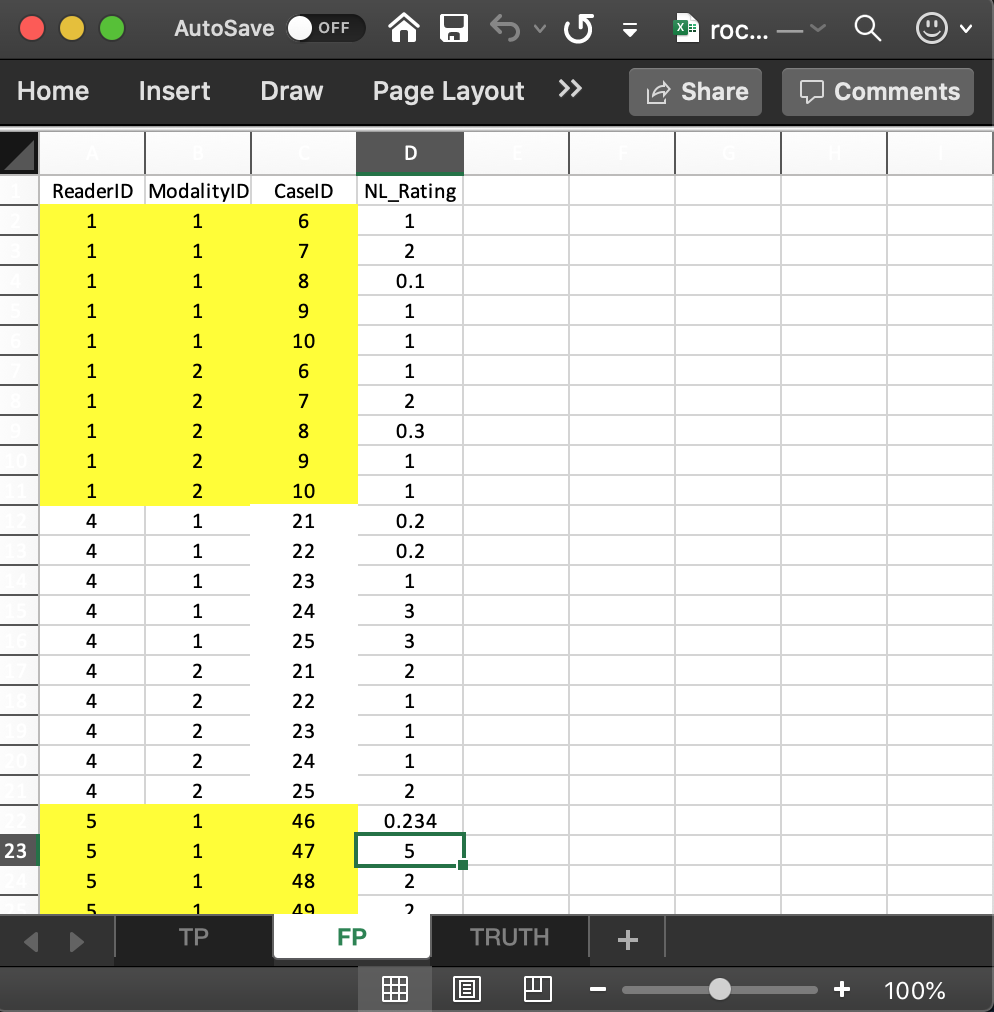
\includegraphics[width=0.5\linewidth,height=0.2\textheight]{images/rocSpFp} 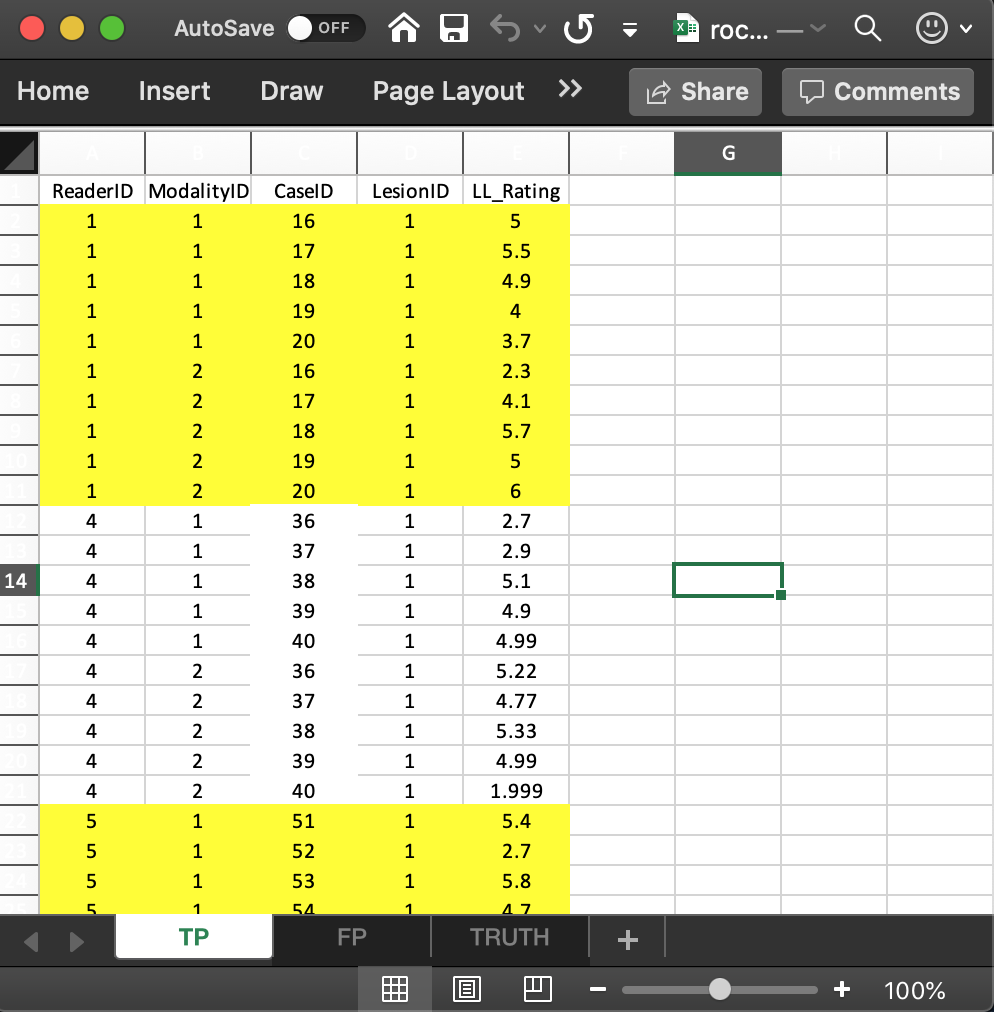
\includegraphics[width=0.5\linewidth,height=0.2\textheight]{images/rocSpTp} 

}

\caption{Fig. 2 FP/TP worksheets; LEFT=FP, (b) RIGHT=TP}\label{fig:unnamed-chunk-9}
\end{figure}

\hypertarget{the-false-positive-fp-ratings-2}{%
\section{The false positive (FP) ratings}\label{the-false-positive-fp-ratings-2}}

\begin{itemize}
\tightlist
\item
  These are found in the \texttt{FP} or \texttt{NL} worksheet, see Fig. 2, left panel.
\item
  This worksheet has the ratings of non-diseased cases.
\item
  The common vertical length is 30 in this example (2 modalities times 3 readers times 5 non-diseased cases per reader).
\item
  \texttt{ReaderID}: the reader labels: these must be from \texttt{1}, \texttt{4} or \texttt{5}, as declared in the \texttt{Truth} worksheet.
\item
  \texttt{ModalityID}: the modality labels: \texttt{1} or \texttt{2}, as declared in the \texttt{Truth} worksheet.
\item
  \texttt{CaseID}: the labels of non-diseased cases. Each \texttt{CaseID} - \texttt{ReaderID} combination must be consistent with that declared in the \texttt{Truth} worsheet.\\
\item
  \texttt{NL\_Rating}: the floating point ratings of non-diseased cases. Each row of this worksheet yields a rating corresponding to the values of \texttt{ReaderID}, \texttt{ModalityID} and \texttt{CaseID} for that row.
\end{itemize}

\begin{Shaded}
\begin{Highlighting}[]
\NormalTok{x}\OperatorTok{$}\NormalTok{NL[,}\DecValTok{1}\NormalTok{,}\DecValTok{1}\OperatorTok{:}\DecValTok{15}\NormalTok{,}\DecValTok{1}\NormalTok{]}
\CommentTok{#>      [,1] [,2] [,3] [,4] [,5] [,6] [,7] [,8] [,9] [,10] [,11] [,12] [,13] [,14]}
\CommentTok{#> [1,]    1    2  0.1    1    1 -Inf -Inf -Inf -Inf  -Inf  -Inf  -Inf  -Inf  -Inf}
\CommentTok{#> [2,]    1    2  0.3    1    1 -Inf -Inf -Inf -Inf  -Inf  -Inf  -Inf  -Inf  -Inf}
\CommentTok{#>      [,15]}
\CommentTok{#> [1,]  -Inf}
\CommentTok{#> [2,]  -Inf}
\NormalTok{x}\OperatorTok{$}\NormalTok{NL[,}\DecValTok{2}\NormalTok{,}\DecValTok{1}\OperatorTok{:}\DecValTok{15}\NormalTok{,}\DecValTok{1}\NormalTok{]}
\CommentTok{#>      [,1] [,2] [,3] [,4] [,5] [,6] [,7] [,8] [,9] [,10] [,11] [,12] [,13] [,14]}
\CommentTok{#> [1,] -Inf -Inf -Inf -Inf -Inf  0.2  0.2    1    3     3  -Inf  -Inf  -Inf  -Inf}
\CommentTok{#> [2,] -Inf -Inf -Inf -Inf -Inf  2.0  1.0    1    1     2  -Inf  -Inf  -Inf  -Inf}
\CommentTok{#>      [,15]}
\CommentTok{#> [1,]  -Inf}
\CommentTok{#> [2,]  -Inf}
\NormalTok{x}\OperatorTok{$}\NormalTok{NL[,}\DecValTok{3}\NormalTok{,}\DecValTok{1}\OperatorTok{:}\DecValTok{15}\NormalTok{,}\DecValTok{1}\NormalTok{]}
\CommentTok{#>      [,1] [,2] [,3] [,4] [,5] [,6] [,7] [,8] [,9] [,10] [,11] [,12] [,13] [,14]}
\CommentTok{#> [1,] -Inf -Inf -Inf -Inf -Inf -Inf -Inf -Inf -Inf  -Inf 0.234     5     2     2}
\CommentTok{#> [2,] -Inf -Inf -Inf -Inf -Inf -Inf -Inf -Inf -Inf  -Inf 3.000     2     2     2}
\CommentTok{#>      [,15]}
\CommentTok{#> [1,]  2.00}
\CommentTok{#> [2,]  0.33}
\end{Highlighting}
\end{Shaded}

\begin{itemize}
\tightlist
\item
  The first line of the above code shows the ratings, in both modalities, of the first five non-diseased cases with \texttt{CaseID}s \texttt{6,7,8,9,10} (indexed 1, 2, 3, 4, 5 and appearing in the first five columns) interpreted by the first reader (\texttt{ReaderID} 1).
\item
  The second line shows the ratings, in both modalities, of the next five non-diseased cases with \texttt{CaseID}s \texttt{21,22,23,24,25} (indexed 6, 7, 8, 9, 10and appearing in the next five columns) interpreted by the second reader (\texttt{ReaderID} 4).
\item
  The third line shows the ratings, in both modalities, of the final five non-diseased cases with \texttt{CaseID}s \texttt{46,47,48,49,50} (indexed 11, 12, 13, 14, 15and appearing in the final five columns) interpreted by the third reader (\texttt{ReaderID} 5).
\item
  Values such as \texttt{x\$NL{[},,16:30,1{]}}, which are there for compatibility with FROC data, are all filled with \texttt{-Inf}.
\end{itemize}

\hypertarget{the-true-positive-tp-ratings-2}{%
\section{The true positive (TP) ratings}\label{the-true-positive-tp-ratings-2}}

\begin{itemize}
\tightlist
\item
  These are found in the \texttt{TP} or \texttt{LL} worksheet, see Fig. 2, right panel.
\item
  This worksheet has the ratings of diseased cases.
\item
  The common vertical length is 30 in this example (2 modalities times 3 readers times 5 diseased cases per reader).
\item
  \texttt{ReaderID}: the reader labels: these must be from \texttt{1}, \texttt{4} or \texttt{5}, as declared in the \texttt{Truth} worksheet.
\item
  \texttt{ModalityID}: the modality labels: \texttt{1} or \texttt{2}, as declared in the \texttt{Truth} worksheet.
\item
  \texttt{CaseID}: the labels of diseased cases. Each \texttt{CaseID} - \texttt{ReaderID} combination must be consistent with that declared in the \texttt{Truth} worsheet.\\
\item
  \texttt{LL\_Rating}: the floating point ratings of diseased cases. Each row of this worksheet yields a rating corresponding to the values of \texttt{ReaderID}, \texttt{ModalityID} and \texttt{CaseID} for that row.
\end{itemize}

\begin{Shaded}
\begin{Highlighting}[]
\NormalTok{x}\OperatorTok{$}\NormalTok{LL[,}\DecValTok{1}\NormalTok{,}\DecValTok{1}\OperatorTok{:}\DecValTok{15}\NormalTok{,}\DecValTok{1}\NormalTok{]}
\CommentTok{#>      [,1] [,2] [,3] [,4] [,5] [,6] [,7] [,8] [,9] [,10] [,11] [,12] [,13] [,14]}
\CommentTok{#> [1,]  5.0  5.5  4.9    4  3.7 -Inf -Inf -Inf -Inf  -Inf  -Inf  -Inf  -Inf  -Inf}
\CommentTok{#> [2,]  2.3  4.1  5.7    5  6.0 -Inf -Inf -Inf -Inf  -Inf  -Inf  -Inf  -Inf  -Inf}
\CommentTok{#>      [,15]}
\CommentTok{#> [1,]  -Inf}
\CommentTok{#> [2,]  -Inf}
\NormalTok{x}\OperatorTok{$}\NormalTok{LL[,}\DecValTok{2}\NormalTok{,}\DecValTok{1}\OperatorTok{:}\DecValTok{15}\NormalTok{,}\DecValTok{1}\NormalTok{]}
\CommentTok{#>      [,1] [,2] [,3] [,4] [,5] [,6] [,7] [,8] [,9] [,10] [,11] [,12] [,13] [,14]}
\CommentTok{#> [1,] -Inf -Inf -Inf -Inf -Inf 2.70 2.90 5.10 4.90 4.990  -Inf  -Inf  -Inf  -Inf}
\CommentTok{#> [2,] -Inf -Inf -Inf -Inf -Inf 5.22 4.77 5.33 4.99 1.999  -Inf  -Inf  -Inf  -Inf}
\CommentTok{#>      [,15]}
\CommentTok{#> [1,]  -Inf}
\CommentTok{#> [2,]  -Inf}
\NormalTok{x}\OperatorTok{$}\NormalTok{LL[,}\DecValTok{3}\NormalTok{,}\DecValTok{1}\OperatorTok{:}\DecValTok{15}\NormalTok{,}\DecValTok{1}\NormalTok{]}
\CommentTok{#>      [,1] [,2] [,3] [,4] [,5] [,6] [,7] [,8] [,9] [,10] [,11] [,12] [,13] [,14]}
\CommentTok{#> [1,] -Inf -Inf -Inf -Inf -Inf -Inf -Inf -Inf -Inf  -Inf   5.4   2.7   5.8   4.7}
\CommentTok{#> [2,] -Inf -Inf -Inf -Inf -Inf -Inf -Inf -Inf -Inf  -Inf   5.4   2.7   5.8   4.7}
\CommentTok{#>      [,15]}
\CommentTok{#> [1,]     5}
\CommentTok{#> [2,]     5}
\end{Highlighting}
\end{Shaded}

\begin{itemize}
\tightlist
\item
  The first line of code shows the ratings, in both modalities, of the first five diseased cases with \texttt{CaseID}s \texttt{16,17,18,19,20} (indexed 1, 2, 3, 4, 5and appearing in the first five columns) interpreted by the first reader (\texttt{ReaderID} 1).
\item
  The second line shows the ratings, in both modalities, of the next five diseased cases with \texttt{CaseID}s \texttt{36,37,38,39,40} (indexed 6, 7, 8, 9, 10and appearing in the next five columns) interpreted by the second reader (\texttt{ReaderID} 4).
\item
  The third line shows the ratings, in both modalities, of the final five non-diseased cases with \texttt{CaseID}s \texttt{51,52,53,54,55} (indexed 11, 12, 13, 14, 15and appearing in the final five columns) interpreted by the third reader (\texttt{ReaderID} 5).
\end{itemize}

\hypertarget{summary-1}{%
\section{Summary}\label{summary-1}}

\begin{itemize}
\tightlist
\item
  The FROC dataset has far less regularity in structure as compared to an ROC dataset.
\item
  The length of the first dimension of either \texttt{x\$NL} or \texttt{x\$LL} list members is the total number of modalities, 2 in the current example.
\item
  The length of the second dimension of either \texttt{x\$NL} or \texttt{x\$LL} list members is the total number of readers, 3 in the current example.
\item
  The length of the third dimension of \texttt{x\$NL} is the total number of cases, 8 in the current example. The first three positions account for \texttt{NL} marks on non-diseased cases and the remaining 5 positions account for \texttt{NL} marks on diseased cases.
\item
  The length of the third dimension of \texttt{x\$LL} is the total number of diseased cases, 5 in the current example.
\item
  The length of the fourth dimension of \texttt{x\$NL} is determined by the case (diseased or non-diseased) with the most \texttt{NL} marks, 2 in the current example.
\item
  The length of the fourth dimension of \texttt{x\$LL} is determined by the diseased case with the most lesions, 3 in the current example.
\end{itemize}

\hypertarget{frocSpdataformat}{%
\chapter{FROC split plot data format}\label{frocSpdataformat}}

\hypertarget{introduction-3}{%
\section{Introduction}\label{introduction-3}}

\begin{itemize}
\tightlist
\item
  The purpose of this vignette is to explain the data format of the input Excel file for an FROC \emph{split-plot} dataset.
\item
  In a split-plot dataset each reader interprets a sub-set of cases in all modalities.
\item
  The cases interpreted by different readers have no overlap.
\item
  It is assumed, for now, that each sub-set of cases has the same numbers of non-diseased and diseased cases.
\end{itemize}

\hypertarget{the-excel-data-format-3}{%
\section{The Excel data format}\label{the-excel-data-format-3}}

The Excel file has three worsheets named \texttt{Truth}, \texttt{NL} or \texttt{FP} and \texttt{LL} or \texttt{TP}.

\hypertarget{the-truth-worksheet-3}{%
\section{\texorpdfstring{The \texttt{Truth} worksheet}{The Truth worksheet}}\label{the-truth-worksheet-3}}

The \texttt{Truth} worksheet contains 6 columns: \texttt{CaseID}, \texttt{LesionID}, \texttt{Weight}, \texttt{ReaderID}, \texttt{ModalityID} and \texttt{Paradigm}.

\begin{itemize}
\tightlist
\item
  The first five columns contain as many rows as there are non-diseased cases (9) plus total number of lesions (27) in the dataset (each row with a non-zero \texttt{LesionID} corresponds to a lesion).
\item
  \texttt{CaseID}: unique \textbf{integers}, one per case, representing the cases in the dataset.
\item
  \texttt{LesionID}: integers 0, 1, 2, etc., with each 0 representing a non-diseased case, 1 representing the \emph{first} lesion on a diseased case, 2 representing the second lesion on a diseased case, if present, and so on.
\item
  The three non-diseased cases interpreted by reader with \texttt{ReaderID} value \texttt{0} are labeled \texttt{1}, \texttt{2}, \texttt{3}, while the diseased cases interpreted by this reader are labeled \texttt{70}, \texttt{71}, \texttt{72}, \texttt{73} and \texttt{74}, with \texttt{LesionID} values ranging from 1 to 3.\\
\item
  The second reader, with \texttt{ReaderID} value \texttt{1}, interprets three non-diseased cases labeled \texttt{4}, \texttt{5} and \texttt{6}, each with \texttt{LesionID} value \texttt{0}, and five diseased cases labeled \texttt{80}, \texttt{81}, \texttt{82}, \texttt{83} and \texttt{84}, with \texttt{LesionID} values ranging from 1 to 3.\\
\item
  The third reader, with \texttt{ReaderID} value \texttt{2}, interprets three non-diseased cases labeled \texttt{7}, \texttt{8} and \texttt{9}, each with \texttt{LesionID} value \texttt{0} and five diseased cases labeled \texttt{90}, \texttt{91}, \texttt{92}, \texttt{93} and \texttt{94}, with \texttt{LesionID} values ranging from 1 to 3.\\
\item
  \texttt{Weight}: floating point value adding upto unity for diseased cases as required for FROC data.
\item
  \texttt{ModalityID}: a comma-separated listing of modalities, each represented by a unique \textbf{integer}. In the example shown below each cell has the value \texttt{0,\ 1}. \textbf{Each cell has to be text formatted.}
\item
  \texttt{Paradigm}: In the example shown below, the contents are \texttt{FROC} and \texttt{split-plot}.
\end{itemize}

\begin{figure}

{\centering 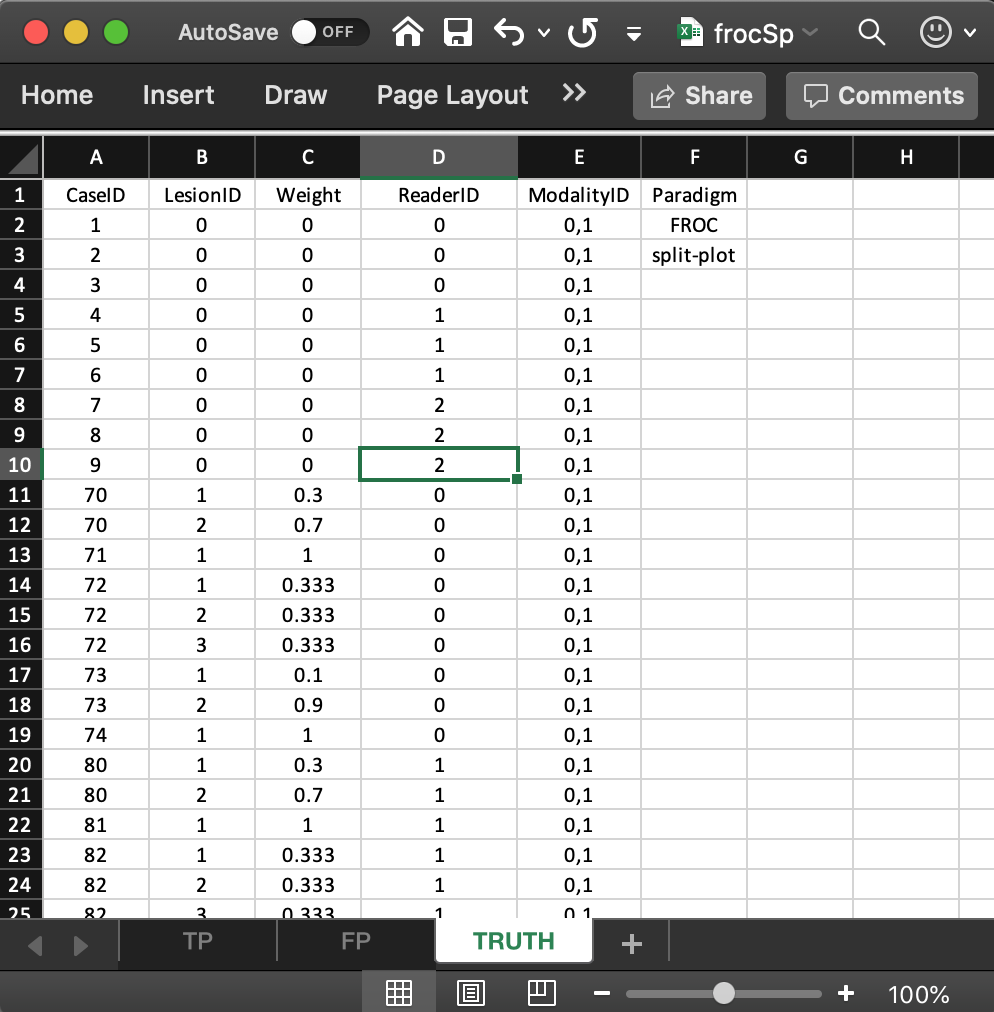
\includegraphics[width=0.5\linewidth,height=0.2\textheight]{images/frocSpTruth} 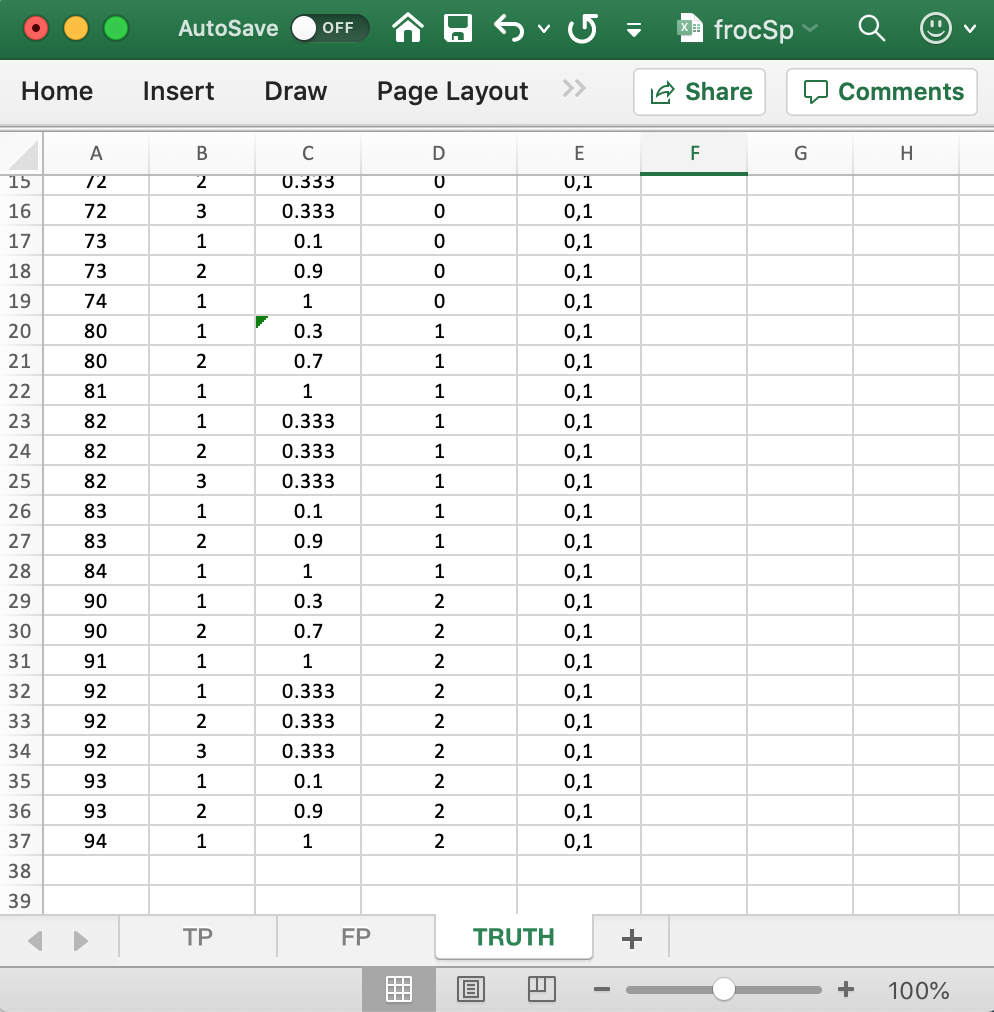
\includegraphics[width=0.5\linewidth,height=0.2\textheight]{images/frocSpTruth2} 

}

\caption{Two views of Truth worksheet for file frocSp.xlsx}\label{fig:frocSpTruth2}
\end{figure}

\hypertarget{the-structure-of-the-froc-split-plot-dataset}{%
\section{The structure of the FROC split plot dataset}\label{the-structure-of-the-froc-split-plot-dataset}}

The example shown in Fig. 1 corresponds to Excel file \texttt{inst/extdata/toyFiles/FROC/frocSp.xlsx} in the project directory.

\begin{Shaded}
\begin{Highlighting}[]
\NormalTok{frocSp <-}\StringTok{ }\KeywordTok{system.file}\NormalTok{(}\StringTok{"extdata"}\NormalTok{, }\StringTok{"toyFiles/FROC/frocSp.xlsx"}\NormalTok{,}
                        \DataTypeTok{package =} \StringTok{"RJafroc"}\NormalTok{, }\DataTypeTok{mustWork =} \OtherTok{TRUE}\NormalTok{)}
\NormalTok{x <-}\StringTok{ }\KeywordTok{DfReadDataFile}\NormalTok{(frocSp, }\DataTypeTok{newExcelFileFormat =} \OtherTok{TRUE}\NormalTok{)}
\KeywordTok{str}\NormalTok{(x)}
\CommentTok{#> List of 12}
\CommentTok{#>  $ NL           : num [1:2, 1:3, 1:24, 1:3] 1.02 2.89 -Inf -Inf -Inf ...}
\CommentTok{#>  $ LL           : num [1:2, 1:3, 1:15, 1:3] 5.28 5.2 -Inf -Inf -Inf ...}
\CommentTok{#>  $ lesionVector : int [1:15] 2 1 3 2 1 2 1 3 2 1 ...}
\CommentTok{#>  $ lesionID     : num [1:15, 1:3] 1 1 1 1 1 1 1 1 1 1 ...}
\CommentTok{#>  $ lesionWeight : num [1:15, 1:3] 0.3 1 0.333 0.1 1 ...}
\CommentTok{#>  $ dataType     : chr "FROC"}
\CommentTok{#>  $ modalityID   : Named chr [1:2] "0" "1"}
\CommentTok{#>   ..- attr(*, "names")= chr [1:2] "0" "1"}
\CommentTok{#>  $ readerID     : Named chr [1:3] "0" "1" "2"}
\CommentTok{#>   ..- attr(*, "names")= chr [1:3] "0" "1" "2"}
\CommentTok{#>  $ design       : chr "SPLIT-PLOT"}
\CommentTok{#>  $ normalCases  : int [1:9] 1 2 3 4 5 6 7 8 9}
\CommentTok{#>  $ abnormalCases: int [1:15] 70 71 72 73 74 80 81 82 83 84 ...}
\CommentTok{#>  $ truthTableStr: num [1:2, 1:3, 1:24, 1:4] 1 1 NA NA NA NA 1 1 NA NA ...}
\end{Highlighting}
\end{Shaded}

\begin{itemize}
\tightlist
\item
  Flag \texttt{newExcelFileFormat} \textbf{must} be set to \texttt{TRUE} for split plot data.
\item
  The dataset object \texttt{x} is a \texttt{list} variable with 12 members.
\item
  Note that the \texttt{dataType} member is FROC and the \texttt{design} member is SPLIT-PLOT.
\item
  There are 15 diseased cases in the dataset (the number of 1's in the \texttt{LesionID} column of the \texttt{Truth} worksheet) and 9 non-diseased cases (the number of 0's in the \texttt{LesionID} column).
\item
  The \texttt{x\$lesionVector} member is a vector with 15 ones representing the 15 diseased cases in the dataset.
\item
  The \texttt{x\$lesionID} member is a 15 x 3 array labeling the lesions in the dataset.
\item
  The \texttt{x\$lesionWeight} member is a 15 x 3 array.
\end{itemize}

\begin{Shaded}
\begin{Highlighting}[]
\NormalTok{x}\OperatorTok{$}\NormalTok{lesionVector}
\CommentTok{#>  [1] 2 1 3 2 1 2 1 3 2 1 2 1 3 2 1}
\NormalTok{x}\OperatorTok{$}\NormalTok{lesionID}
\CommentTok{#>       [,1] [,2] [,3]}
\CommentTok{#>  [1,]    1    2 -Inf}
\CommentTok{#>  [2,]    1 -Inf -Inf}
\CommentTok{#>  [3,]    1    2    3}
\CommentTok{#>  [4,]    1    2 -Inf}
\CommentTok{#>  [5,]    1 -Inf -Inf}
\CommentTok{#>  [6,]    1    2 -Inf}
\CommentTok{#>  [7,]    1 -Inf -Inf}
\CommentTok{#>  [8,]    1    2    3}
\CommentTok{#>  [9,]    1    2 -Inf}
\CommentTok{#> [10,]    1 -Inf -Inf}
\CommentTok{#> [11,]    1    2 -Inf}
\CommentTok{#> [12,]    1 -Inf -Inf}
\CommentTok{#> [13,]    1    2    3}
\CommentTok{#> [14,]    1    2 -Inf}
\CommentTok{#> [15,]    1 -Inf -Inf}
\NormalTok{x}\OperatorTok{$}\NormalTok{lesionWeight}
\CommentTok{#>            [,1]      [,2]      [,3]}
\CommentTok{#>  [1,] 0.3000000 0.7000000      -Inf}
\CommentTok{#>  [2,] 1.0000000      -Inf      -Inf}
\CommentTok{#>  [3,] 0.3333333 0.3333333 0.3333333}
\CommentTok{#>  [4,] 0.1000000 0.9000000      -Inf}
\CommentTok{#>  [5,] 1.0000000      -Inf      -Inf}
\CommentTok{#>  [6,] 0.3000000 0.7000000      -Inf}
\CommentTok{#>  [7,] 1.0000000      -Inf      -Inf}
\CommentTok{#>  [8,] 0.3333333 0.3333333 0.3333333}
\CommentTok{#>  [9,] 0.1000000 0.9000000      -Inf}
\CommentTok{#> [10,] 1.0000000      -Inf      -Inf}
\CommentTok{#> [11,] 0.3000000 0.7000000      -Inf}
\CommentTok{#> [12,] 1.0000000      -Inf      -Inf}
\CommentTok{#> [13,] 0.3333333 0.3333333 0.3333333}
\CommentTok{#> [14,] 0.1000000 0.9000000      -Inf}
\CommentTok{#> [15,] 1.0000000      -Inf      -Inf}
\end{Highlighting}
\end{Shaded}

\begin{itemize}
\tightlist
\item
  The \texttt{x\$truthTableStr} member is a \texttt{2\ x\ 3\ x\ 24\ x\ 4} array, i.e., I x J x K x (maximum number of lesions per case plus 1). The \texttt{plus\ 1} is needed to accommodate normal cases with \texttt{lesionID} = 0.
\item
  Each entry in this array is either \texttt{1}, meaning the corresponding interpretation exists, or \texttt{NA}, meaning the corresponding interpretation does not exist.
\item
  For example, \texttt{x\$truthTableStr{[}1,1,1,1{]}} is 1. This means that an interpretation exists for the first treatment (\texttt{modalityID} = 0), first reader (\texttt{readerID} = 0) and first (normal) case \texttt{caseID} = 1 and \texttt{lesionID} = 0. This example corresponds to row 2 in the \texttt{TRUTH} worksheet.
\item
  \texttt{x\$truthTableStr{[}1,1,4,1{]}} is NA, which means an interpretation does not exist for the first treatment, first reader and fourth (normal) case.
\item
  However, \texttt{x\$truthTableStr{[}1,2,4,1{]}} is 1, which means an interpretation does exist for the first treatment, second reader and fourth (normal) case. This example corresponds to row 5 in the \texttt{TRUTH} worksheet.
\item
  Likewise, \texttt{x\$truthTableStr{[}1,1,10,3{]}} is 1, which means an interpretation does exist for the first treatment, first reader, tenth (abnormal) case and \texttt{lesionID} = 2. This example corresponds to row 12 in the \texttt{TRUTH} worksheet.
\item
  As an aside, in the FROC paradigm an interpretation need not yield a mark-rating pair. An interpretation means the reader was ``exposed to'' and had the opportunity to mark the corresponding treatment-reader-case-lesion combination.
\item
  The reader should confirm that the contents of \texttt{x\$truthTableStr} summarizes the structure of the data in the \texttt{TRUTH} worksheet.
\end{itemize}

\hypertarget{the-false-positive-fp-ratings-3}{%
\section{The false positive (FP) ratings}\label{the-false-positive-fp-ratings-3}}

These are found in the \texttt{FP} or \texttt{NL} worksheet, see Fig. 2.

\begin{figure}

{\centering 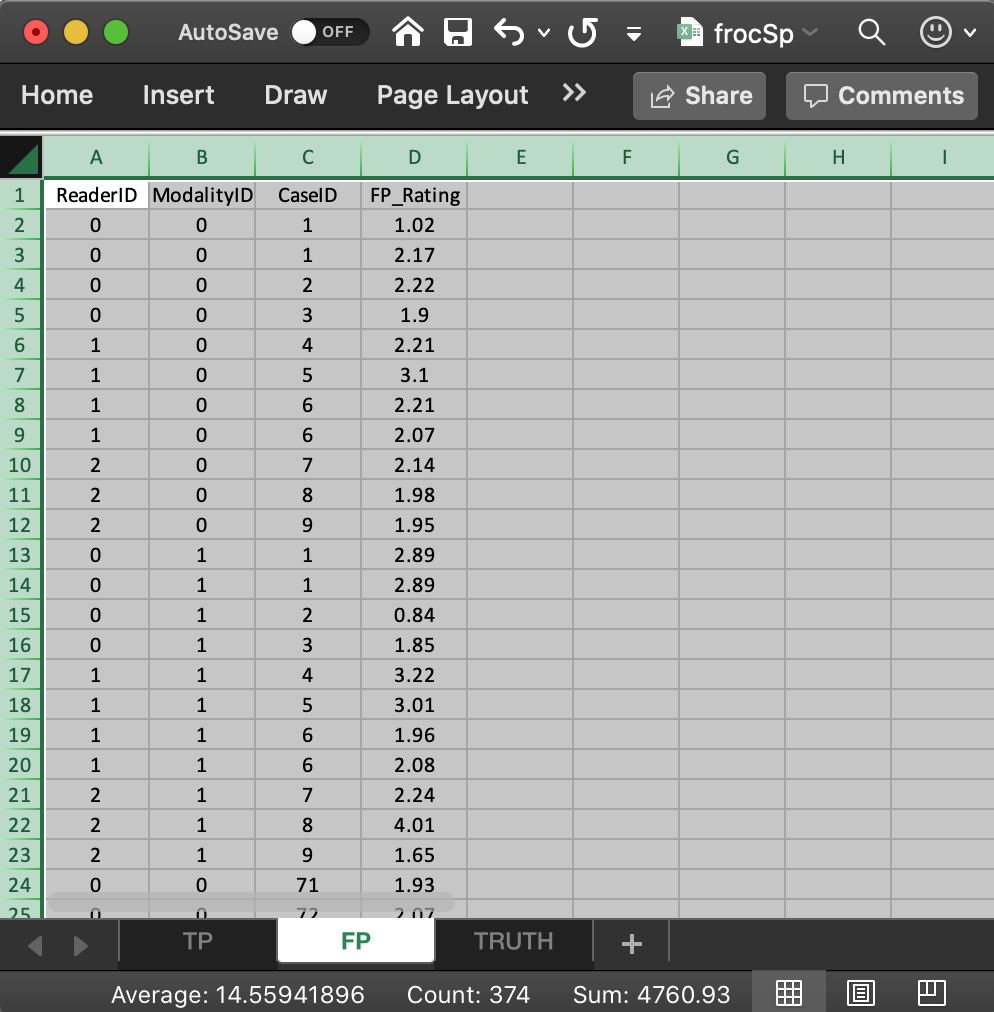
\includegraphics[width=0.5\linewidth,height=0.2\textheight]{images/frocSpNL} 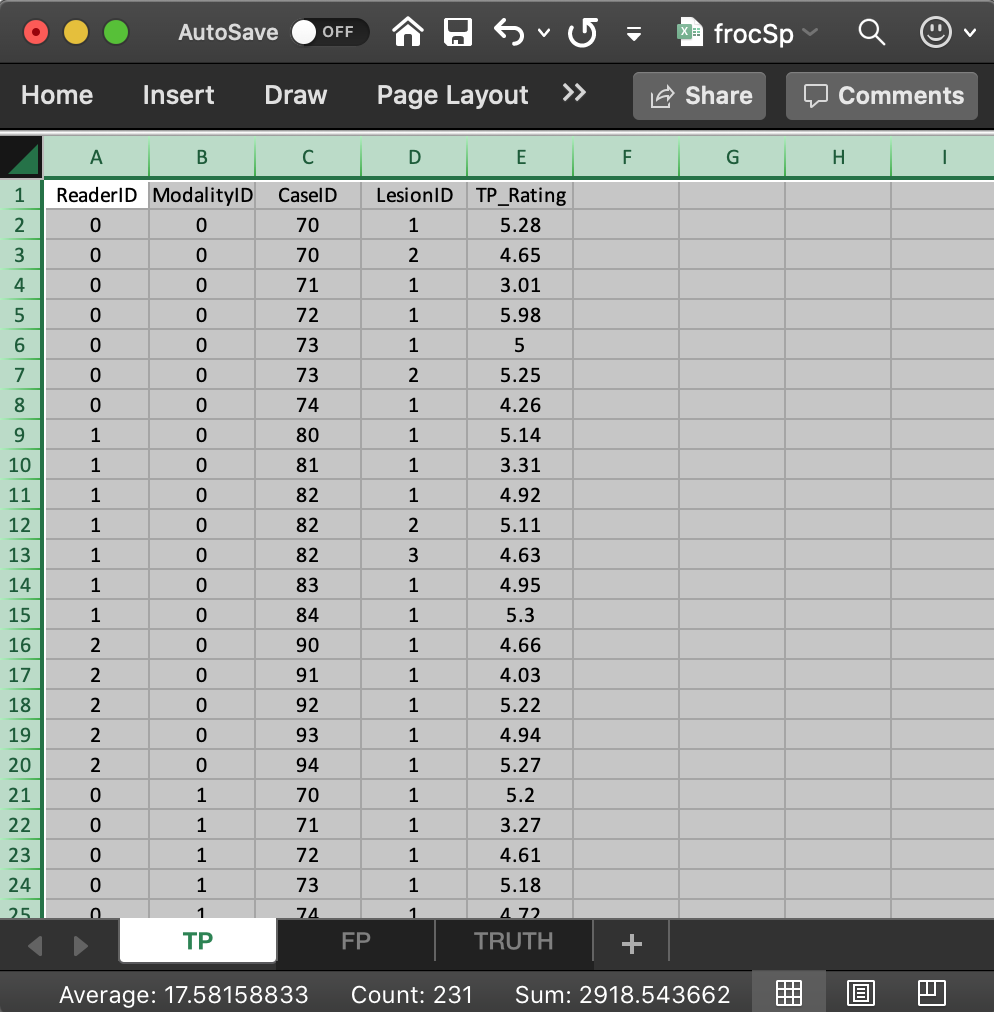
\includegraphics[width=0.5\linewidth,height=0.2\textheight]{images/frocSpLL} 

}

\caption{NL/FP worksheet, left, and LL/TP worksheet, right, for file frocSp.xlsx}\label{fig:frocSpLL}
\end{figure}

\begin{itemize}
\tightlist
\item
  This worksheet has the ratings of non-diseased cases.
\item
  The common vertical length is 30 in this example (2 modalities times 3 readers times 5 non-diseased cases per reader).
\item
  \texttt{ReaderID}: the reader labels: these must be from \texttt{0}, \texttt{1} or \texttt{2}, as declared in the \texttt{Truth} worksheet.
\item
  \texttt{ModalityID}: the modality labels: \texttt{0} or \texttt{1}, as declared in the \texttt{Truth} worksheet.
\item
  \texttt{CaseID}: the labels of non-diseased cases. Each \texttt{CaseID}, \texttt{ModalityID}, \texttt{ReaderID} combination must be consistent with that declared in the \texttt{Truth} worsheet.\\
\item
  \texttt{FP\_Rating}: the floating point ratings of non-diseased cases. Each row of this worksheet yields a rating corresponding to the values of \texttt{ReaderID}, \texttt{ModalityID} and \texttt{CaseID} for that row. Each \texttt{CaseID}, \texttt{ModalityID}, \texttt{ReaderID} combination must be consistent with that declared in the \texttt{Truth} worsheet.
\end{itemize}

\begin{Shaded}
\begin{Highlighting}[]
\NormalTok{x}\OperatorTok{$}\NormalTok{NL[,}\DecValTok{1}\NormalTok{,}\DecValTok{1}\OperatorTok{:}\DecValTok{9}\NormalTok{,}\DecValTok{1}\NormalTok{]}
\CommentTok{#>      [,1] [,2] [,3] [,4] [,5] [,6] [,7] [,8] [,9]}
\CommentTok{#> [1,] 1.02 2.22 1.90 -Inf -Inf -Inf -Inf -Inf -Inf}
\CommentTok{#> [2,] 2.89 0.84 1.85 -Inf -Inf -Inf -Inf -Inf -Inf}
\NormalTok{x}\OperatorTok{$}\NormalTok{NL[,}\DecValTok{2}\NormalTok{,}\DecValTok{1}\OperatorTok{:}\DecValTok{9}\NormalTok{,}\DecValTok{1}\NormalTok{]}
\CommentTok{#>      [,1] [,2] [,3] [,4] [,5] [,6] [,7] [,8] [,9]}
\CommentTok{#> [1,] -Inf -Inf -Inf 2.21 3.10 2.21 -Inf -Inf -Inf}
\CommentTok{#> [2,] -Inf -Inf -Inf 3.22 3.01 1.96 -Inf -Inf -Inf}
\NormalTok{x}\OperatorTok{$}\NormalTok{NL[,}\DecValTok{3}\NormalTok{,}\DecValTok{1}\OperatorTok{:}\DecValTok{9}\NormalTok{,}\DecValTok{1}\NormalTok{]}
\CommentTok{#>      [,1] [,2] [,3] [,4] [,5] [,6] [,7] [,8] [,9]}
\CommentTok{#> [1,] -Inf -Inf -Inf -Inf -Inf -Inf 2.14 1.98 1.95}
\CommentTok{#> [2,] -Inf -Inf -Inf -Inf -Inf -Inf 2.24 4.01 1.65}
\end{Highlighting}
\end{Shaded}

\begin{itemize}
\tightlist
\item
  The first line of the above code shows the ratings, in both modalities, of the first three non-diseased cases with \texttt{CaseID}s \texttt{1,3,3} (indexed 1, 2, 3 and appearing in the first three columns) interpreted by the first reader (\texttt{ReaderID} \texttt{0}).
\item
  The second line shows the ratings, in both modalities, of the next three non-diseased cases with \texttt{CaseID}s \texttt{4,5,6} (indexed 4, 5, 6and appearing in the next three columns) interpreted by the second reader (\texttt{ReaderID} \texttt{1}).
\item
  The third line shows the ratings, in both modalities, of the final three non-diseased cases with \texttt{CaseID}s \texttt{7,8,9} (indexed 7, 8, 9and appearing in the final three columns) interpreted by the third reader (\texttt{ReaderID} \texttt{2}).
\item
  Values such as \texttt{x\$NL{[},,16:30,1{]}}, which are there for compatibility with FROC data, are all filled with \texttt{-Inf}.
\end{itemize}

\hypertarget{the-true-positive-tp-ratings-3}{%
\section{The true positive (TP) ratings}\label{the-true-positive-tp-ratings-3}}

These are found in the \texttt{TP} or \texttt{LL} worksheet, see below.

\begin{itemize}
\tightlist
\item
  This worksheet has the ratings of diseased cases.
\item
  The common vertical length is 30 in this example (2 modalities times 3 readers times 5 diseased cases per reader).
\item
  \texttt{ReaderID}: the reader labels: these must be from \texttt{0}, \texttt{1} or \texttt{2}, as declared in the \texttt{Truth} worksheet.
\item
  \texttt{ModalityID}: the modality labels: \texttt{0} or \texttt{1}, as declared in the \texttt{Truth} worksheet.
\item
  \texttt{CaseID}: the labels of diseased cases. Each \texttt{CaseID}, \texttt{ModalityID}, \texttt{ReaderID} combination must be consistent with that declared in the \texttt{Truth} worsheet.\\
\item
  \texttt{TP\_Rating}: the floating point ratings of diseased cases. Each row of this worksheet yields a rating corresponding to the values of \texttt{ReaderID}, \texttt{ModalityID} and \texttt{CaseID} for that row. Each \texttt{CaseID}, \texttt{ModalityID}, \texttt{ReaderID} combination must be consistent with that declared in the \texttt{Truth} worsheet.
\end{itemize}

\begin{Shaded}
\begin{Highlighting}[]
\NormalTok{x}\OperatorTok{$}\NormalTok{LL[,}\DecValTok{1}\NormalTok{,}\DecValTok{1}\OperatorTok{:}\DecValTok{15}\NormalTok{,}\DecValTok{1}\NormalTok{]}
\CommentTok{#>      [,1] [,2] [,3] [,4] [,5] [,6] [,7] [,8] [,9] [,10] [,11] [,12] [,13] [,14]}
\CommentTok{#> [1,] 5.28 3.01 5.98 5.00 4.26 -Inf -Inf -Inf -Inf  -Inf  -Inf  -Inf  -Inf  -Inf}
\CommentTok{#> [2,] 5.20 3.27 4.61 5.18 4.72 -Inf -Inf -Inf -Inf  -Inf  -Inf  -Inf  -Inf  -Inf}
\CommentTok{#>      [,15]}
\CommentTok{#> [1,]  -Inf}
\CommentTok{#> [2,]  -Inf}
\NormalTok{x}\OperatorTok{$}\NormalTok{LL[,}\DecValTok{2}\NormalTok{,}\DecValTok{1}\OperatorTok{:}\DecValTok{15}\NormalTok{,}\DecValTok{1}\NormalTok{]}
\CommentTok{#>      [,1] [,2] [,3] [,4] [,5] [,6] [,7] [,8] [,9] [,10] [,11] [,12] [,13] [,14]}
\CommentTok{#> [1,] -Inf -Inf -Inf -Inf -Inf 5.14 3.31 4.92 4.95  5.30  -Inf  -Inf  -Inf  -Inf}
\CommentTok{#> [2,] -Inf -Inf -Inf -Inf -Inf 4.77 3.19 5.20 5.39  5.01  -Inf  -Inf  -Inf  -Inf}
\CommentTok{#>      [,15]}
\CommentTok{#> [1,]  -Inf}
\CommentTok{#> [2,]  -Inf}
\NormalTok{x}\OperatorTok{$}\NormalTok{LL[,}\DecValTok{3}\NormalTok{,}\DecValTok{1}\OperatorTok{:}\DecValTok{15}\NormalTok{,}\DecValTok{1}\NormalTok{]}
\CommentTok{#>      [,1] [,2] [,3] [,4] [,5] [,6] [,7] [,8] [,9] [,10] [,11] [,12] [,13] [,14]}
\CommentTok{#> [1,] -Inf -Inf -Inf -Inf -Inf -Inf -Inf -Inf -Inf  -Inf  4.66  4.03  5.22  4.94}
\CommentTok{#> [2,] -Inf -Inf -Inf -Inf -Inf -Inf -Inf -Inf -Inf  -Inf  4.87  1.94  -Inf  -Inf}
\CommentTok{#>      [,15]}
\CommentTok{#> [1,]  5.27}
\CommentTok{#> [2,]  4.78}
\end{Highlighting}
\end{Shaded}

\begin{itemize}
\tightlist
\item
  The first line of code shows the ratings, in both modalities, of the first five diseased cases with \texttt{CaseID}s \texttt{70,71,72,73,74} (indexed 1, 2, 3, 4, 5 and appearing in the first five columns) interpreted by the first reader (\texttt{ReaderID} \texttt{0}).
\item
  The second line shows the ratings, in both modalities, of the next five diseased cases with \texttt{CaseID}s \texttt{80,81,82,83,84} (indexed 6, 7, 8, 9, 10 and appearing in the next five columns) interpreted by the second reader (\texttt{ReaderID} \texttt{1}).
\item
  The third line shows the ratings, in both modalities, of the final five non-diseased cases with \texttt{CaseID}s \texttt{90,91,92,93,94} (indexed 11, 12, 13, 14, 15 and appearing in the final five columns) interpreted by the third reader (\texttt{ReaderID} \texttt{2}).
\end{itemize}

\hypertarget{summary-2}{%
\section{Summary}\label{summary-2}}

\begin{itemize}
\tightlist
\item
  TBA
\end{itemize}

\bibliography{packages.bib,myRefs.bib}

\end{document}
